% !TEX encoding = IsoLatin
\documentclass[12pt, a4paper]{article}
\usepackage[utf8]{inputenc}
\usepackage{lmodern}
\usepackage[T1]{fontenc}
%\usepackage[latin1]{inputenc}
\usepackage[hmargin = 25mm, vmargin = 25mm]{geometry}
%\geometry{letterpaper}                   % ... or a4paper or a5paper or ... 
%\geometry{landscape}                % Activate for for rotated page geometry
%\usepackage[parfill]{parskip}    % Activate to begin paragraphs with an empty line rather than an indent
\usepackage{graphicx}
\usepackage{amssymb, amsmath, amsthm}
\usepackage{epstopdf}
\usepackage{moreverb,stmaryrd}
\usepackage{natbib}
\usepackage[nottoc,notlot,notlof]{tocbibind}
\usepackage{hyperref}
\usepackage{algorithm,algorithmic}
%\usepackage[french]{babel}
\usepackage{hyperref}
\usepackage{fancyhdr} 
\usepackage{booktabs}
\usepackage{longtable}
\usepackage{array}
\usepackage{multirow}
\usepackage[table]{xcolor}
\usepackage{wrapfig}
\usepackage{float}
\usepackage{colortbl}
\usepackage{pdflscape}
\usepackage{tabu}
\usepackage{threeparttable}
\usepackage{threeparttablex}
\usepackage{makecell}

\pagestyle{fancy}
\renewcommand{\headrulewidth}{0pt}
\fancyhead[C]{} 
\fancyhead[L]{}
\fancyhead[R]{}

\renewcommand{\footrulewidth}{0pt}
\fancyfoot[C]{
\thepage
%\footnotesize{$13^{es}$ Journées de méthodologie statistique de l’Insee (JMS) / 12-14 juin 2018 / PARIS}
}
\fancyfoot[R]{%\thepage
}

\begin{document}
\newcommand{\inter}[2]{\llbracket  #1\,,\, #2  \rrbracket}
\pagenumbering{roman}

\begin{center}
\line(1,0){450}
\vspace{5mm}
\textbf{
(In)Stability of Reg-ARIMA Models for Seasonal Adjustment
}
\end{center}

\vspace{5mm}
\small{{\bf keywords}: seasonal adjustment, calendar effects, Reg-ARIMA models, outliers.}

\begin{center}
\line(1,0){450}
\end{center}


\section*{Abstract}

Regression models with ARIMA errors (Reg-ARIMA) are nowadays commonly used in seasonal adjustment to remove the main deterministic effects (outliers, ruptures, calendar effects) from the raw data before decomposing the corrected series into trend-cycle, seasonality and irregular.

The main seasonal adjustment programs (\textsc{X-13Arima-Seats}, \textsc{Tramo-Seats}, \textsc{JDemetra+}) implement these models in an automatic and very user-friendly way. This facility hides in fact a real complexity and in certain cases a lack of robustness which can escape the user.

In this presentation, we draw attention to the real difficulties of implementing these models through concrete cases: the estimation of a leap year effect, the estimation of breaks and even the estimation of an ARIMA model.

\newpage

\tableofcontents

\newpage


\listoftables
\listoffigures

\newpage

\pagenumbering{arabic}
\section*{Introduction \markboth{Introduction}{Introduction}}
\addcontentsline{toc}{section}{Introduction} 

The most popular seasonal adjustment methods are undoubtedly \textsc{Tramo-Seats} (\cite{GM1996} and \cite{MC2004}), a parametric method based on ARIMA models and \textsc {X-13Arima-Seats} (\cite{FMBOC1998} and \cite{LQ2001}), a non-parametric method based on moving averages.
Both methods are recommended by Eurostat and the European Central Bank (ECB) for the seasonal adjustment of economic indicators.

These methods proceed in two steps summarized in figure~\ref{fig:X13TS}. First, they adjust the raw series from some deterministic effects (outliers, breaks, calendar effects) and, in a second step, they decompose the series thus ``cleaned'' into trend-cycle, seasonal component and irregular component.

\begin{figure}[!ht]
\begin{center}
 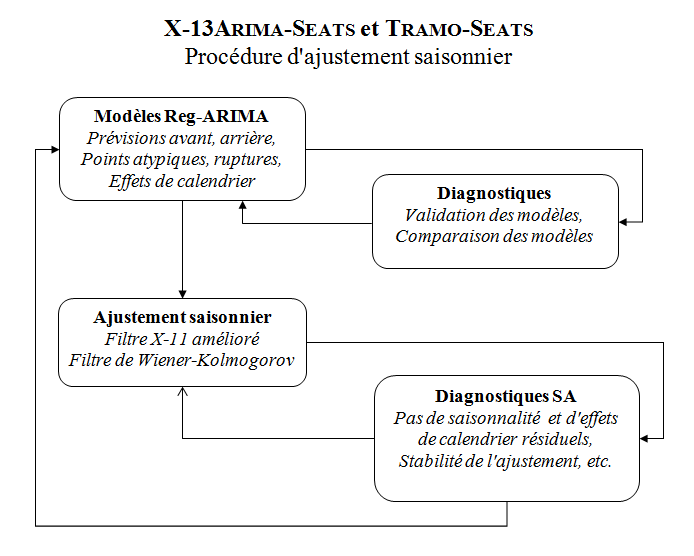
\includegraphics[scale=0.8]{img/MethodesX13-TS.png}
 \caption{The seasonal adjustment process of \textsc{X-13Arima-Seats} and \textsc{Tramo-Seats}: correction and decomposition.}
 \label{fig:X13TS}
\end{center}
\end{figure}

The pre-decomposition stage, called pre-adjustment, is based on a ``regression model with ARIMA errors'' (Reg-ARIMA model). An automatic modeling algorithm (AMI) is available to the user that allows to:

\begin{itemize}
  \item determine the mode of the model (additive or multiplicative);
	\item detect and correct breaks in the series; 
	\item detect and correct potel calendar effects (trading day effects and moving holidays such as Easter);
	\item adjust the ``residuals'' of the regression with an ARIMA model;
	\item estimate any missing values;
	\item and finally to forecast and backcast the series studied.
\end{itemize}

This automatic algorithm is implemented in a very user-friendly in softwares and it always comes with a large battery of statistical tests to judge the quality of the adjustment made. A very detailed description can be found in \cite{GM1998}.

\cite{MLP2015}, \cite{MLP2016}, \cite{M2018} assess the performances of this AMI. Their results are laudatory for this tool but they consider, on the one hand, a modeling at a given moment and they validate, on the other hand, the method by the tests which finally served to build it. Nevertheless, the AMI is a first-rate \textbf{exploratory} tool, unfortunately too often used in practice as a black box.

\vskip \baselineskip
The goal of this article is, based on simple simulations on real data and focusing on the stability of estimates, to show that these Reg-ARIMA models are complex, difficult to use, and must be handled with caution.

In the first part, we briefly remind the definition of Reg-ARIMA models and the main deterministic components used in this work. The second part of the study is devoted to the estimate of the leap year effect in the industrial production index (IPI) and the turnover index (ITI) series of countries of the European Union. The third part focuses in the estimation of four kinds of outliers --- additive outliers, transitory change, level shift and seasonal outliers --- in the IPI series. The fourth part looks at the estimates of the ARIMA model itself.

This article does not \textbf{prove} anything: it is settle for \textbf{showing} on concrete examples, that the modelization Reg-ARIMA suffers, like number of parametric methods, of a certain lack of robustness. The use of these models, also very powerful, requires both a good knowledge of the underlying theory and its limits, and great caution as well summarized \cite{FMcE2018}:

\begin{quote}
``\textit{ARIMA Model-Based Seasonal Adjustment (AMBSA) should not be a black box procedure to its users because default software procedures are sometimes seriously inadequate. Also user decisions regarding software options and model choice can strongly impact the results obtained, for better or worse. A seasonal adjuster who understands the basic facets of the method and some of its diagnostics, as outlined and then detailed in this document, will have a greater capacity to obtain successful adjustments}''.
\end{quote}

\vskip \baselineskip
The proper use of these models also requires a bit of common sense. Thus, and by way of example, it is certainly absurd to try to correctly estimate a leap year effect with a model on a series of less than 9 years old. To estimate this effect, you will have observed only two leap years, which is very little.

\section{Reg-ARIMA models}

\subsection{Definition}

Let $z_t$ an observed time series, monthly ($s=12$) or quaterly ($s=4$) and if necessary log-transformed. \textsc{X-13Arima-Seats} and \textsc{Tramo-Seats} adjust $z_t$ a model:
\begin{equation}
 \begin{array}{lcl}
   z_t & = & y'_t\beta + x_t \\
	\phi(B)x_t & = & \Theta(B)  a_t,
 \end{array}
 \label{eq:eq1}
\end{equation}
Where:
\begin{itemize}
	\item $y'_t\beta$ is the part of the regression that takes into account the deterministic components of the series;
	\item $x_t$, the ``residuals'', follows an ARIMA model $(p,d,q)(P,D,Q)_s$;
	\item $\phi(B)$ and $\Theta(B)$ are polynomials of the lag operator $B$ ($B^j  z_t=z_{t-j}$);
	\item and $a_t$ is a white noise.
\end{itemize}
\vskip \baselineskip
For seasonal series, a multiplicative specification is used:
\begin{equation}
	\varphi_r (B) \varphi_s (B^s ) \nabla^D \nabla_s^{D_s}   x_t = \theta_r (B) \theta_s (B^s)  a_t,
	\label{eq:eq2}
\end{equation}
where:
\begin{itemize}
	\item ($\nabla^D, \nabla_s^{D_s}$) is the differentiation that leads to stationarity, with $\nabla^D = (1-B)^D$ and $\nabla^{D_s}_s=(1-B^s)^{D_s}$,
	\item $\varphi_r (B)$  and $\varphi_s (B^s)$ are the autoregressive polynomials associated with the regular and seasonal stationary components, order $P_r$ and $P_s$: 
$$
\begin{array}{lcl}
\varphi_r (B)   & = & 1 + \varphi_{r,1} (B) + \cdots + \varphi_{r,P_r} (B^{P_r}) \\
\varphi_s (B^s) & = & 1 + \varphi_{s,1} (B^s) + \cdots + \varphi_{s,P_s} (B^{sP_s}),
\end{array}
$$
	\item $\theta_r (B)$  and $\theta_s (B^s)$ are the moving average polynomials associated with the regular and seasonal components, order $Q_r$ and $Q_s$: 
$$
\begin{array}{lcl}
\theta_r (B)   & = & 1 + \theta_{r,1} (B) + \cdots + \theta_{r,Q_r} (B^{Q_r}) \\
\theta_s (B^s) & = & 1 + \theta_{s,1} (B^s) + \cdots + \theta_{s,Q_s} (B^{sQ_s}),
\end{array}
$$
	\item and $a_t$ is a white noise.
\end{itemize}

In the automatic algorithm implemented by \textsc{X-13Arima-Seats} and \textsc{Tramo-Seats}, the orders of the polynomials are constrained: $P_r\text{ and }Q_r\in \inter{0}{3}$, $D\in \inter{0}{2}$ and $D_s$, $P_s$ and $Q_s\in \inter{0}{1}$, which corresponds to 384 possibles ARIMA models. 

\subsection{The deterministic componets of the regression}

In seasonal adjustment, we usually focus on two important components: calendar effects, which must be suppressed in the series ``seasonally adjusted and working days adjusted'' (SA-WDA) and the presence of breaks that may hinder the estimate of the seasonal component.

\subsubsection{The calendars effects}

The different calendars effects, the associated models and the problems related to their detection and estimation are detailed in \cite{L2018}. Here we focus on the so-called ``working days'' effects linked to the fact that the composition in days of the month --- the numbers of Mondays, Tuesdays, \dots, Sundays --- varies over time.

Following the notations of \cite{FMBOC1998}, we assume that the day number $j$ of the week has an effect $\alpha_j$ where, for example, $j=1$ means Monday, $j=2$  Tuesdays, \dots and $j=7$ means Sunday. For instance, each $\alpha_j$ represents the average sales of day $j$. If $N_{jt}$ number of days $j$ during the month $t$, the length of the month $t$ is then $N_t = \sum_{j=1}^{j=7} N_{jt}$ and the cumulative effect for this month (the total sales of the month) will be:
$TD_t = \sum_{j=1}^{j=7} \alpha_j N_{jt}$.

A first idea to detect and estimate the working days effects in a series is to explain the values of the series by the seven variables $N_{jt} $. However, these regressors are naturally seasonal (there are on average more Mondays in January than in February) and strongly correlated.

A different but equivalent specification makes it possible to resolve these problem to a large extent. The average daily effect, average saled for a day, is $\bar{\alpha} = \sum_{j=1}^7 \alpha_j /7$. 
By construction $\sum_{j=1}^7 \left(\alpha_j-\bar{\alpha}\right) = 0$, and we have:
\begin{eqnarray*}
\sum_{j=1}^7 \alpha_j N_{jt} & = & \bar{\alpha}N_t + \sum_{j=1}^7 \left(\alpha_j-\bar{\alpha}\right) N_{jt} \nonumber \\
& = &  \bar{\alpha}N_t + \sum_{j=1}^6 \left(\alpha_j-\bar{\alpha}\right) \left(N_{jt} - N_{7t}\right).
\end{eqnarray*}
Thus, the cumulative effect of the month is composed of an effect directly related to the length of the month and a net effect of each day of the week. Since the quantity $ \bar{\alpha} N_t $ is seasonal by nature (January always has more days than February), we use the equality: $\bar{\alpha}N_t = \bar{\alpha}N_t^* + \bar{\alpha}\left(N_t-N_t^*\right)$, where $N_t^*$
is the average of the month of length $t$. In other words, $N_t^*$ is equal to $30$ or $31$ if the month in question is not a February and $28.25$\footnote {In fact, the true value would be $28.2425 $ as shown in the appendix (\ref{sec:cal}).} otherwise. The second term of equality is therefore null except for the month of February. The use of the contrasts variables thus allows seasonal adjustment of the regressors working days.

Current versions of \textsc{X-13Arima-Seats} and \textsc{Tramo-Seats} use the following Reg-ARIMA model to estimate trading days effects:
\begin{eqnarray}
	\label{eq:eq3}
z_t=\beta_0 LY_t + \sum_{j=1}^{j=6} \beta_j \left(N_{jt} - N_{7t}\right) + x_t,
\end{eqnarray}
where $LY_t$ is the leap year (LY) regressor equals to:
\[
LY_{t} = \left\{ \begin{array}{rl} 
                0.75 & \mbox{if } t \mbox{ is a February during leap years} \\
                -0.25 & \mbox{if } t \mbox{ is a February during non leap years} \\
                0 & \mbox{otherwise}
               \end{array}
         \right.
\]


\subsubsection{Outliers and breaks}
\label{sec:PAR}

The different outliers, the associated models and the problems related to their detection and estimate are described in detail in \cite{Me2018}.

In the continuation, we will will focus on the following breaks:
\begin{itemize}
	\item An additive outlier ($AO$), a break affecting only one observation $t_0$, one month. $AO$ are modeled with the following regressor: 
	
$
AO_{t} = \left\{ \begin{array}{cl} 
                1 & \mbox{if } t=t_{0} \\
                0 & \mbox{if } t\neq t_{0}
               \end{array}
       \right.
$
	\item A level shift ($LS$), representing a permanent break in the level of the series from the time $t_0$. $LS$ are modeled with the following regressor: 
	
$
LS_{t} = \left\{ \begin{array}{rl} 
                -1 & \mbox{if } t<t_{0} \\
                0 & \mbox{if } t\geq t_{0}
               \end{array}
       \right.
$
	\item A transitory change ($TC$), a break on a given time $t_0$ that decays exponentially over the following periods. $TC$ are modeled with the following regressor: 
	
$
TC_{t} = \left\{ \begin{array}{cl} 
                0 & \mbox{if } t<t_{0} \\
                \alpha^{t-t_{0}} & \mbox{if } t \geq t_{0}
               \end{array}
       \right.
$

where $\alpha$, which is the speed back to normal, is by default equals to 0.7.
	\item A seasonal outlier ($SO$), an abrupt change in the seasonal pattern of a given month. $SO$ are modeled with the following regressor: 
	
$			
SO_{t} = \left\{ \begin{array}{cl} 
                0 & \mbox{if } t \geq t_{0} \\
								1 & \mbox{if } t < t_{0} \mbox{ and } t  \mbox{ is the same month/quarter of } t_{0}\\
                -1/(s-1) & \mbox{otherwise }
               \end{array}
       \right.		
$
\end{itemize}

\vskip \baselineskip

Figure~\ref{fig:Outliers} gives a graphical representation of the regressors associated with these four breaks.

AO and LS are relatively common in economic series. SO and TC are much rarer and often difficult to explain from an economic point of view. Other types of breaks are sometimes considered: ramps ($RP$), temporary level changes $TLS$\dots


\begin{figure}[!ht]
\begin{center}
 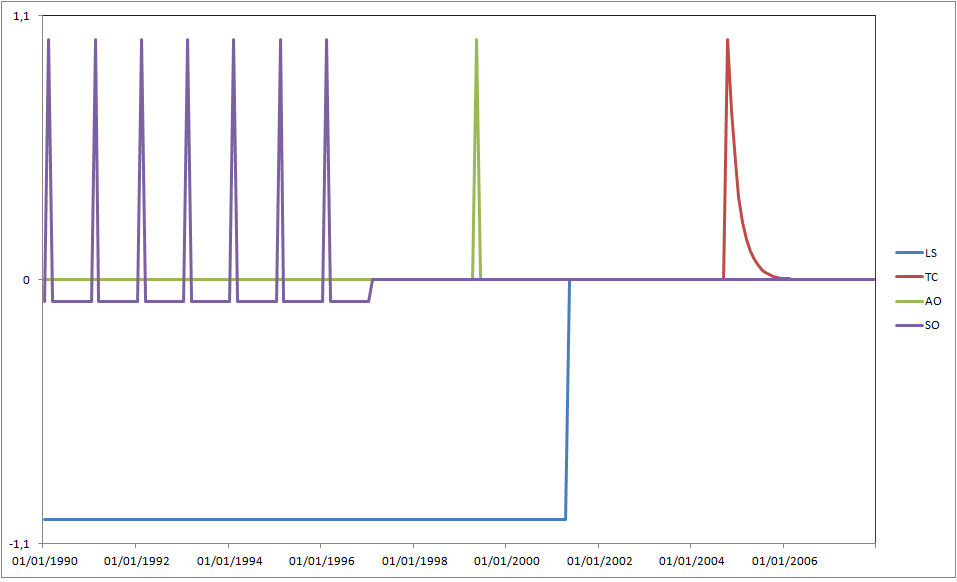
\includegraphics[scale=0.65]{img/Outliers.png}
 \caption{Regressors associated with some kind of breaks (AO, LS, TC, SO).}
 \label{fig:Outliers}
\end{center}
\end{figure}


\subsection{An example \textsc{X-13Arima-Seats}}

As an example, figure~\ref{fig:IPI} shows the result of an automatic modelling on the IPI of the French manufacturing industry, from January 2006 to April 2017. Computations were made with the software  \textsc{JDemetra+}\footnote{\textsc{JDemetra+} is the seasonal adjustment software officially recommended to the members of the European Statistical System (ESS) and the European System of Central Banks. In particular, it implements the methods \textsc{X-13Arima-Seats} and \textsc{Tramo-Seats}.} version 2.2.1, using the Reg-ARIMA module implemented in \textsc{X-13Arima-Seats} and and the default pre-defined specification ``RSA5c'', see \cite{G2017} for more information.

All the statistical indicators associated to the computations are ``green'' (i.e.: considered ``good'' by \textsc{JDemetra+}) and the final model shows:
\begin{itemize}
	\item A strong working days effect with a negative estimate coefficient expected for the weekend;
	\item A leap year effect;
	\item A more surprising Easter effect;
	\item An additive outlier in May 2011 when the production seems to have been much stronger than expected.
\end{itemize}
When these deterministic effects are removed, the series follows an Airline model $(0,1,1)(0,1,1)$.

\vskip \baselineskip

This simple example highlights some of the limitations of a ``blind'' use of the AMI: Why would industrial production fall in the week before Easter? The use of the ``RSA5c'' option is equivalent to specify a specific Reg-ARIMA model and in particular to consider that the IPI is affected by the Easter holiday. If this hypothesis could be eventually accepted for some sectors (lamb meat, chocolate production), it seems harebrained at the global level. On the other hand, some sectors of the retail trade could have an Easter effect (sale of chocolate, lamb, flowers).

The AMI, which automatically implements the Box and Jenkins method, helps the analyst to formulate, \textbf{to specify}, a model by revealing to him the possible presence of outliers and breaks, of calendar effects and by proposing an ARIMA model for the residuals of this model. This algorithm is particularly useful for starting an analysis, especially when one has to deal with tens or hundreds of series. It is also sometimes used in an annual seasonal adjustment campaign to check if the models used in production could not be substituted by others.

It must be understood and kept in mind that this tool is exploratory. Despite its exceptional effectiveness, it is not a confirmatory tool and its results have no character of absolute truth. It's easy to show that: 
\begin{itemize}
	\item In practice, it often happens that the model proposed by the AMI is modified to: include atypical points or breaks, change the system of regressors for working days, even modify the ARIMA model, etc.
	\item It is not uncommon that \textsc{Seats} reject the ARIMA model proposed by \textsc{Tramo} to choose a decomposable model.
	\item The AMI algorithms of \textsc{X13-Arima-Seats} and \textsc{Tramo-Seats} are different and give different results. By way of illustration, both algorithms were appied on 205 IPI's series: the ARIMA model is not the same in 60\% of the cases and the diagnosis on the significance of the working days set of regressors is different for 10\% of the series (see table~\ref{table:CompareTSX13}).
	\item These algorithms use many statistical tests and are very sensitive to preprogrammed threshold values. Thus, changing the default value of the significance test for atypical points can have very important consequences for the final proposed model.
\end{itemize}

\begin{table}
\caption[Comparison of the results of the AMI for X13-Arima-Seats and Tramo-Seats on the 205 IPI series (6 trading days regressors and leap year regressors)]{Comparison of the results of the AMI for \textsc{X13-Arima-Seats} and \textsc{Tramo-Seats} on the 205 IPI series (6 trading days regressors and leap year regressors).}\label{table:CompareTSX13}
\begin{center}
\small
\begin{tabular}{lrr} \\
\hline
\rule{0pt}{3ex}Result&Model& Trading day diagnostic?  \\
\hline
Different&  84&  22 \\
Identical& 121& 183 \\
\hline
Total& 205 & 205  \\
\hline
\end{tabular}
\normalsize
\end{center}
\end{table}

We will now illustrate some problems related to a ``blind use'' of this algorithm by focusing on the stability and relevance of the Reg-ARIMA model estimates.

\begin{figure}[!ht]
\begin{center}
 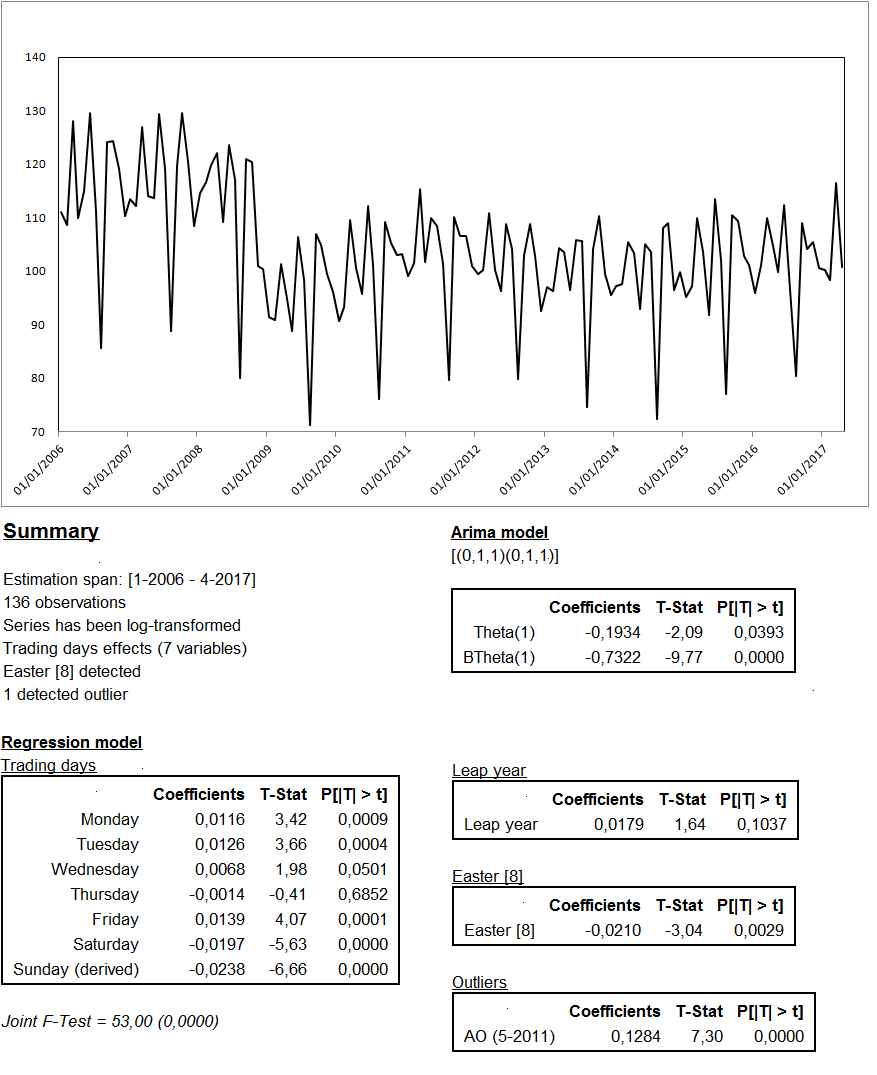
\includegraphics[scale=0.7]{img/IPImanuf.png}
 \caption[Automatic modeling of the IPI of the French manufacturing industry]{Automatic modeling of the IPI of the French manufacturing industry.}
 \label{fig:IPI}
\end{center}
\end{figure}

\clearpage

\section{Estimate of a leap year effect}
\label{sec:LY}

As shown by the equation \ref{eq:eq3}), the leap year effect is a component of the working day effect generated by the composition in days of the month, variable from one year and one month to the other.

The presence of trading days regressors in the Reg-ARIMA model implies, on the one hand, that these effects exist, and ,on the other hand, that they are largely independent of the ARIMA model\footnote{Is to ensure as much as possible this independence that the regressors are seasonally adjusted (this is one of the advantages of considering contrasts).}, and finally that they are constant over time.

Apart from the assumption of independence, these hypothesis can only be validated putting the series back  to their real context. For that matter, the seasonal adjustment guidelines, \cite{E2015}, specifies that:

{\it ``The calendar adjustment should be done for those time series for which there is an economic rationale for the existence of calendar effects and statistical evidence.''}

In this study we assume that industrial production and turnover indices are impacted by calendar effects. This is undoubtedly true because these effects result from various laws or branch agreements: compulsory weekly breaks, usually on Sundays, legal holidays, etc. But on the one hand, there are many possible adjustments and, on the other hand, industries adapt their production process to make it less sensitive to holidays, weekends, holidays, etc. In practice, it is also easy to check that the weekend is a period of low industrial production and that Saturday is a very favorable day for turnover of retail businesses.

Likewise, it is obvious that there is a leap year effect in all series that measure a monthly activity as a sum of daily activities\footnote{However, it is possible that this economic ``evidence'' is disturbed by the statistical collection itself. Thus, in the context of the IPI, some productions are, or have been, measured in whole production units. In the case of the manufacture of aircraft or steamers, it is certain that the leap year effect would not be discernible because of a bias related to the truncation of the measure at monthly level. This kind of problem is less common since worked or billed hours are increasingly used.}. One extra day can only increase the production or the turnover, and whatever the model Reg-ARIMA and associated tests say: on average, this increase will be of $(29/28 - 1) =  0.0357$ so around 3.6\%. \cite{B1992} explains this figure for a multiplicative model and even proposes in this case to make a prior adjustment for the leap year effect rather than to estimate it in a Reg-ARIMA model, which gave rise to the \emph{autoadjust} option of \textsc{X13-Arima-Seats}.

\subsection{Methodology}

In this study on the quality of the estimates of the leap year effect, we use the monthly industrial production and turnover indices in volume, at the 2, 3 or 4-digit levels of the NACE rev 2. To study the convergence of the estimates, we only keep series of more than 12 years. In total, 2198 series are used in the simulation\footnote{These series are available on the Eurostat website, in the tables \emph{sts\_intv\_m}, \emph{sts\_setu\_m}, \emph{sts\_sepr\_m} and \emph{sts\_inpr\_m}. \url{http://ec.europa.eu/eurostat/data/database}.}.

For each series, we proceed as follows:
\begin{enumerate}
	\item In a first step, the decomposition model, the atypical points, the breaks, the  working days effects and the ARIMA model are determined on the whole series. The Reg-ARIMA model is therefore determined.
	\item In a second step, the Reg-ARIMA model is re-estimated on the first 48 observations of the series, to be certain to observe at least one leap year.
	\item Finally, the process is repeated by adding an observation each time, which gives new estimates of the parameters. For a 13-year series, we will therefore have  $12\times 13 - 48 = 108$ estimates of the coefficient of the leap year variable.
\end{enumerate}
These simulations make it possible to study the convergence of the leap year coefficient. In this study, we will say that the estimate of the leap year coefficient has converged when it remains positive, statistically significant and not significantly different from the last estimate (obtained estimating the model with all the data).

Other specifications are of course possible for this simulation: shortening the initial estimation period, not fixing the model, etc. We have conducted different experiments that lead to similar results. Only the results of this simulution with a fixed Reg-ARIMA model are presented here.

\subsection{Results}
In the estimation of this leap year effect, a Reg-ARIMA model is naturally confronted with several difficulties:
\begin{itemize}
	\item The lack of data: to identify the effect of a leap year, we must observe leap years\dots{} and enough.
	\item The difficulty of isolating each component, we remind that they are not observed directly, especially when the series is very noisy.
\end{itemize}

The main results are well summarized in the figures \ref{fig:LYexemple1} and \ref{fig:LYexemple2}; in these figures, the shaded areas represent the 90\% and 95\% confidence intervals.
\begin{itemize}
	\item In both cases, we see that the leap year coefficient takes time to converge and the values of the first years are particularly erratic.
	\item The first leap year is observed here in 1992, and the others in 1996, 2000, 2004, etc. It is only from 2004 that the coefficient converges for the series RF0610; convergence is much slower for the series RF1391.
	\item The estimated values for the RF1391 series are not economically justifiable: how could one more day in a month increase production, all other things being equal, from 7\% to 14\%, or even 19\%?
\end{itemize}

\begin{figure}[!ht]
\begin{center}
 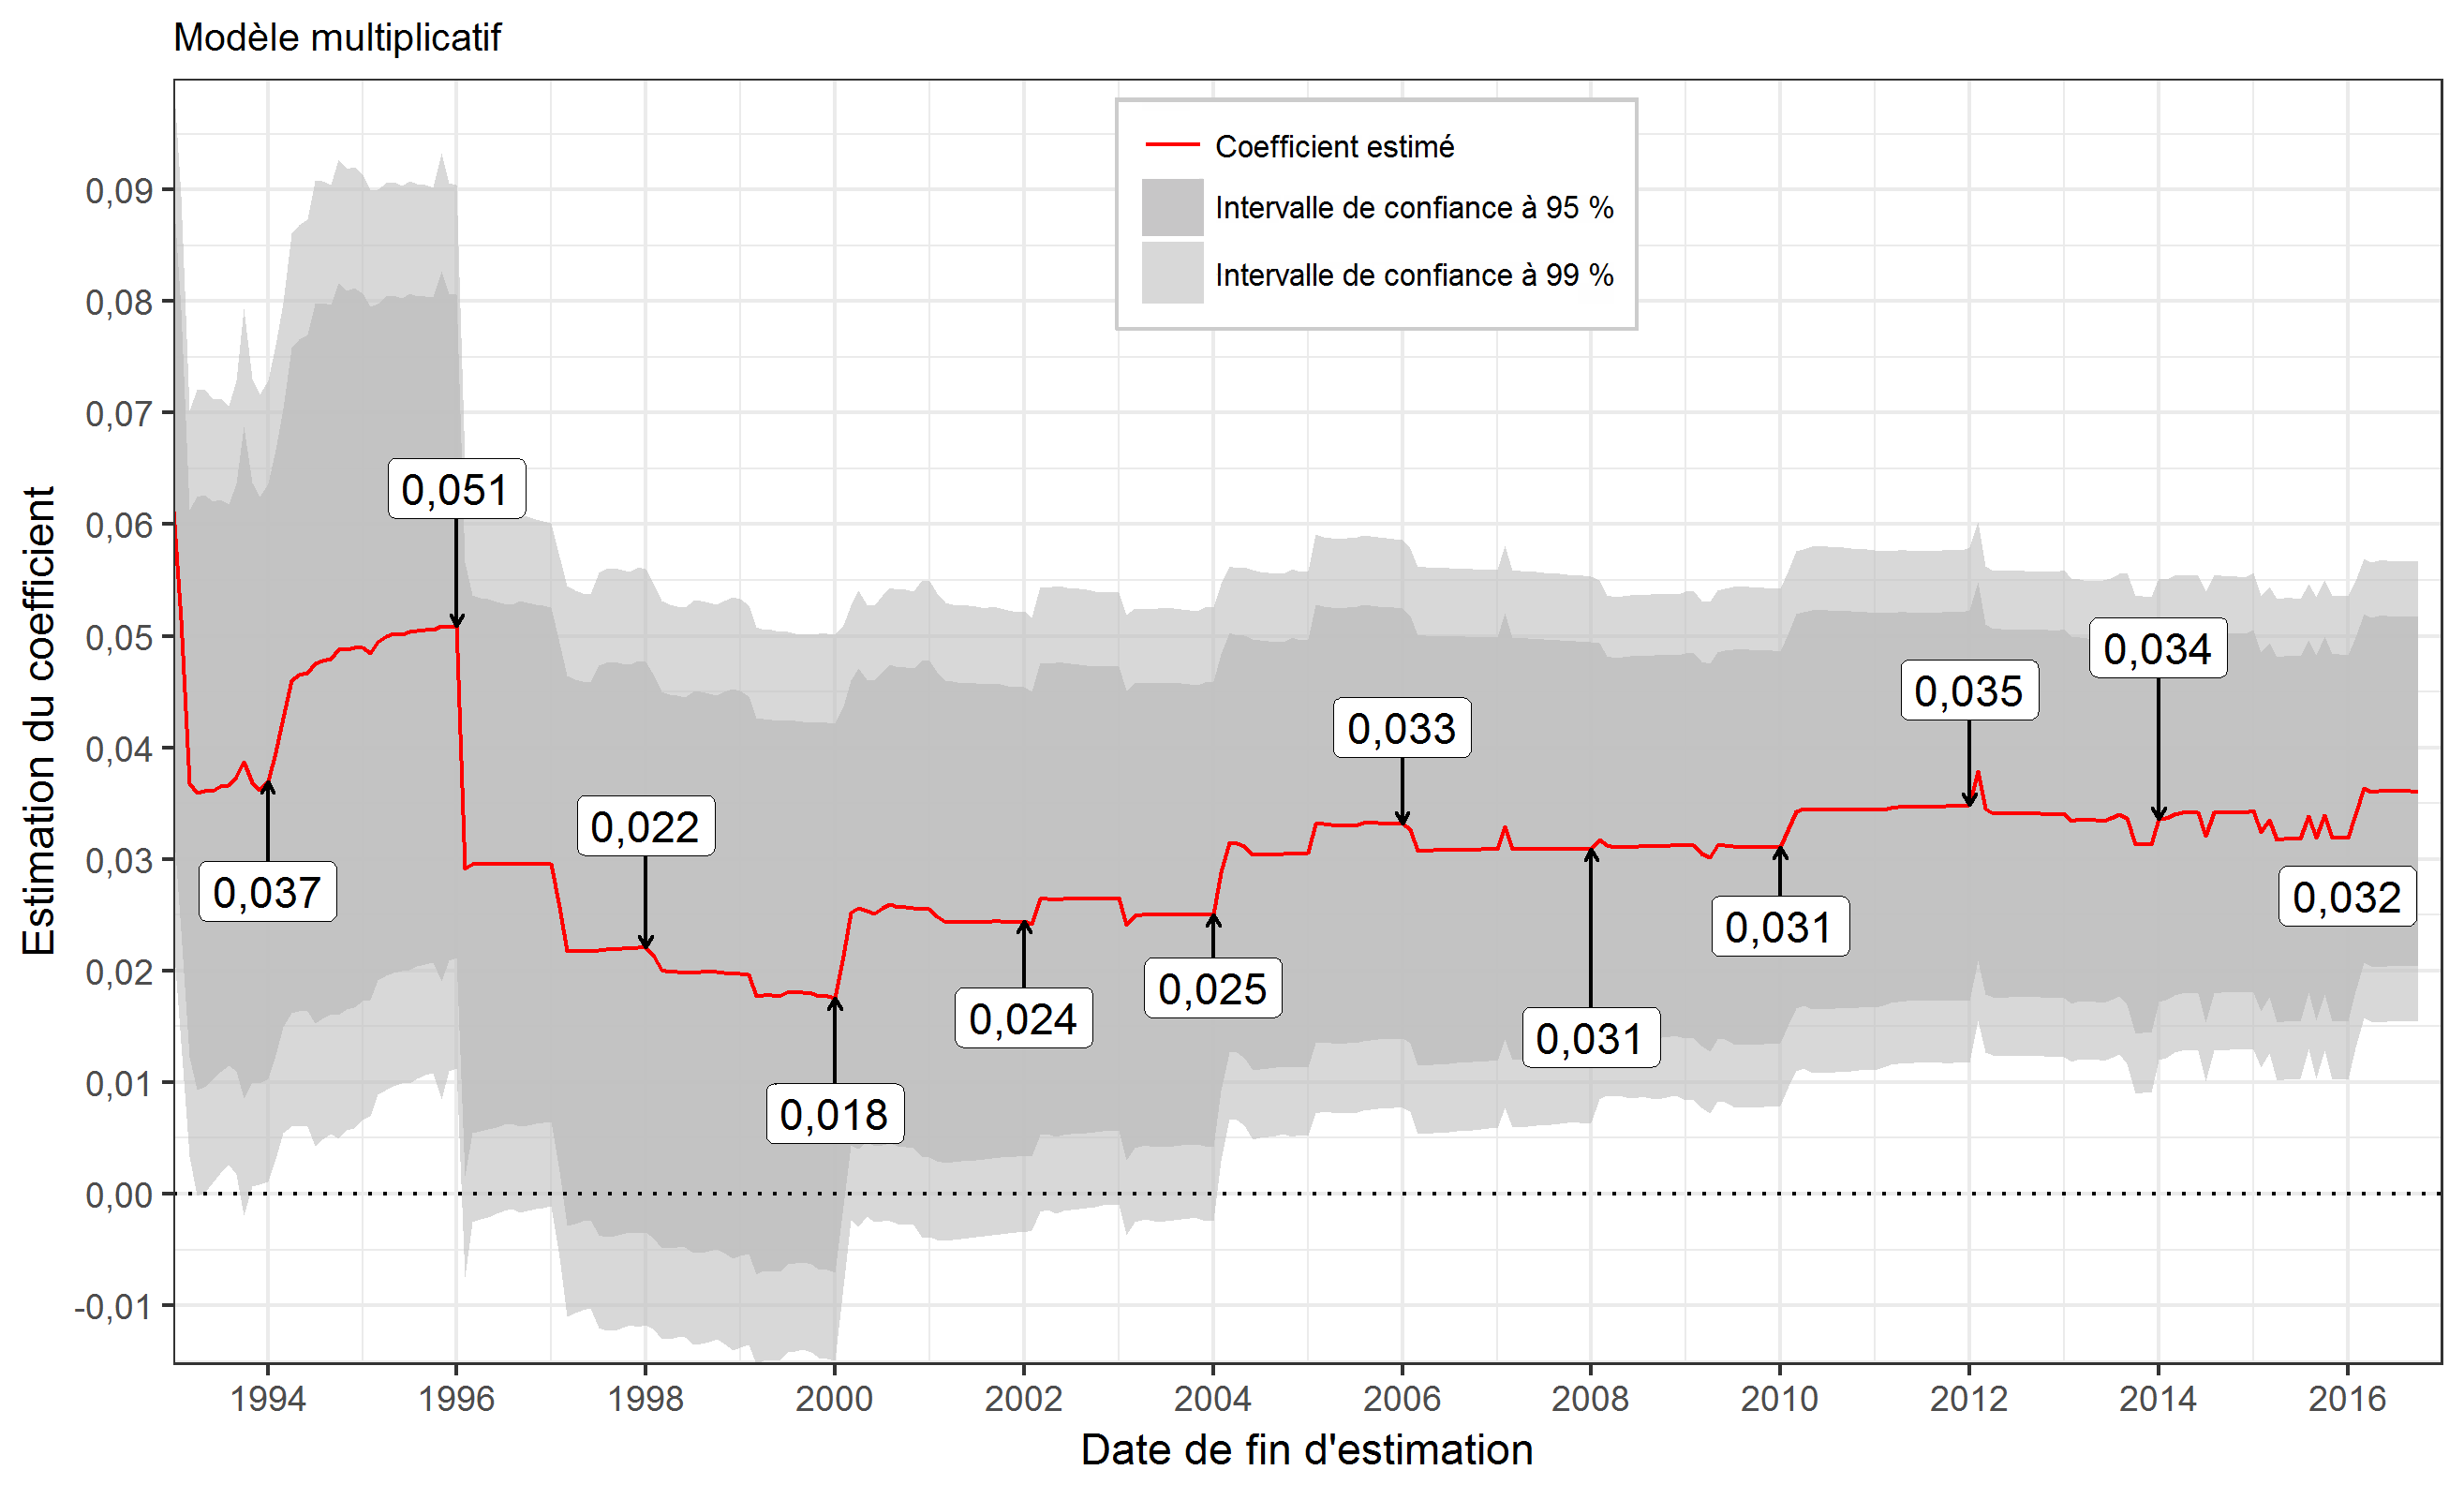
\includegraphics[scale=0.50]{img/LYexemple1.png}
 \caption[Successive estimates of the leap year coefficient for the series RF0610 (extraction of crude
petroleum)]{Successive estimates of the leap year coefficient for the series RF0610 (extraction of crude
petroleum).}
 \label{fig:LYexemple1}
\end{center}
\end{figure}

\begin{figure}[!ht]
\begin{center}
 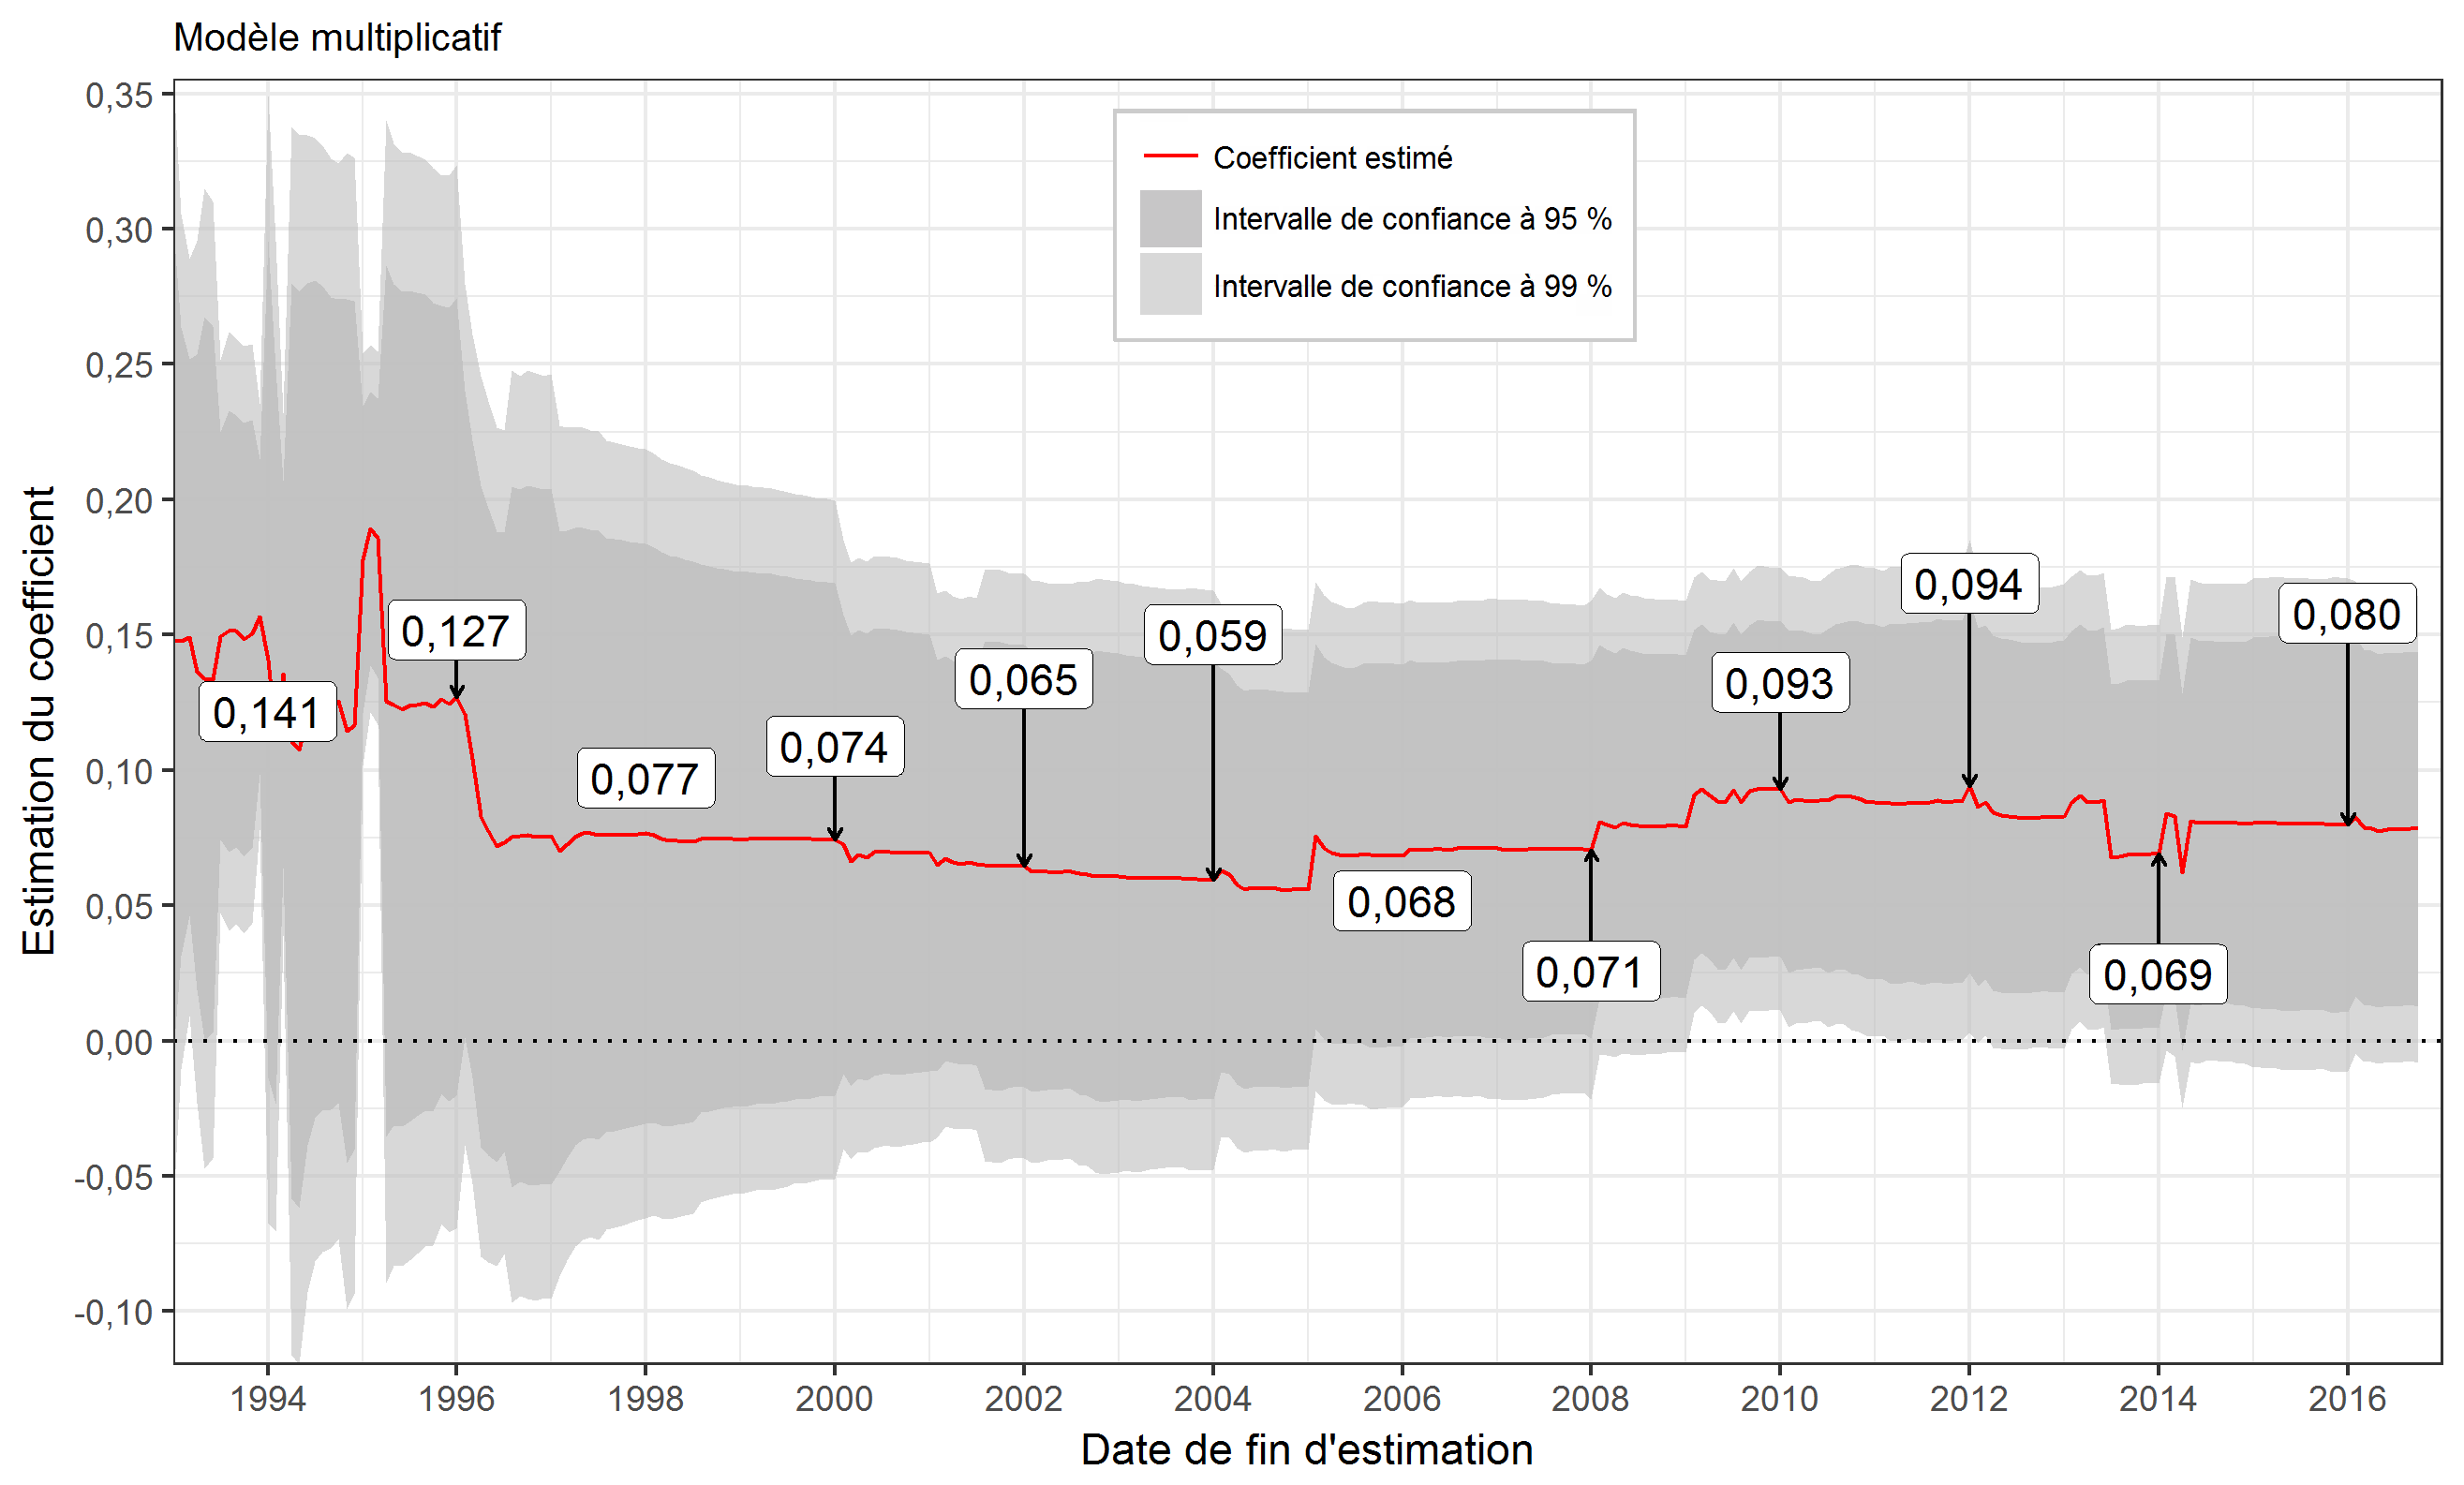
\includegraphics[scale=0.50]{img/LYexemple2.png}
 \caption[Successive estimates of the leap year coefficient for the series RF139 (manufacture of
knitted and crocheted fabrics)]{Successive estimates of the leap year coefficient for the series RF1391 (manufacture of
knitted and crocheted fabrics).}
 \label{fig:LYexemple2}
\end{center}
\end{figure}
The convergence indicators have been calculated \emph{in fine} on 624 series. The figures \ref{fig:LYconvergence} and \ref{fig:LYvaleur} summarize the results of the simulation, in the form of ``violins'': the violins are variants of the boxplots. The shape of the box represent the distribution and the horizontal lines are the corresponding quartiles.


In terms of time needed to obtain a stable estimate, the figure \ref{fig:LYconvergence}) suggests that:
\begin{itemize}
	\item For three-quarters of the series, it takes at least 10 years for the leap year effect to converge. It is a simple question of common sense: below 3 observations, it is most often impossible to measure with fiability a phenomenon, here the difference between the months of February of normal years and leap years.
		\item The nature of the model, additive or multiplicative, has little influence on the time convergence.
	\item Convergence seems faster for turnover series than for industrial production series.
\end{itemize}

\begin{figure}[!ht]
\begin{center}
 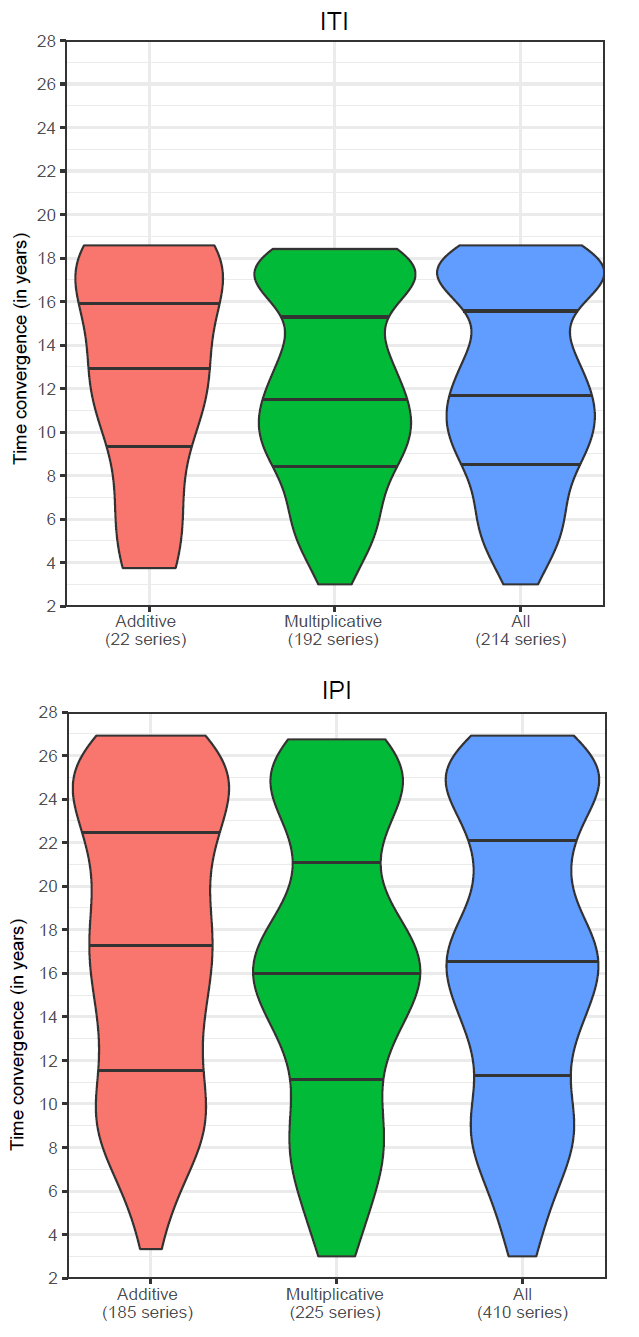
\includegraphics[scale=0.65]{img/LYconvergence2.png}
 \caption[Time convergence (in years) of the leap year coefficient (study on 624 series)]{Time convergence (in years) of the leap year coefficient (study on 624 series).}
 \label{fig:LYconvergence}
\end{center} \vspace{-0.3cm}
\footnotesize
\emph{
Reading note: on the ordinate, the probability density of the time convergence of the estimate of the leap year regressor. The horizontal lines represent the associated quartiles (minimum, first quartile, median, third quartile and maximum).}
\end{figure}

Regarding the value of the coefficient, the figure \ref{fig:LYvaleur} suggests that:
\begin{itemize}
	\item For multiplicative models, turnover indices (ITI) converge to a median value close to the expected value ($3.5\%$) as \cite{B1992} underlines. However, for the IPI, the median value is higher, close to 0.45 point.
	\item For the additive models, the ITI series converge in median to 3 index points, which approximately corresponds to the expected value since the indices are not in general very different from 100. On the other hand, for the IPI, this median value is higher, close 4.5 points.
	\item For many series, about 20\%, the estimate value seems excessive: beyond 6 points and sometimes much more.
\end{itemize}

\begin{figure}[!ht]
\begin{center}
 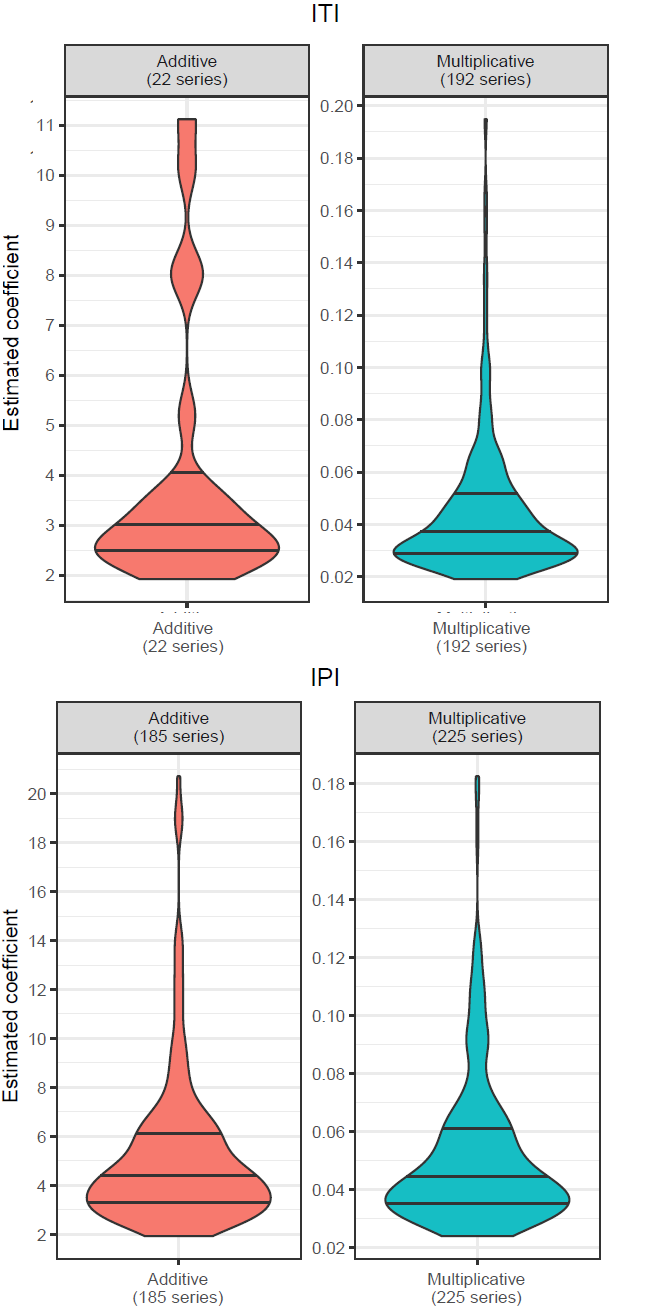
\includegraphics[scale=0.65]{img/LYvaleur2.png}
 \caption[Final estimate of the leap year effect (study on 624 series)]{Final estimate of the leap year effect (study on 624 series).}
 \label{fig:LYvaleur}
\end{center}
\vspace{-0.3cm}
\footnotesize\emph{%
Reading note: on the ordinate, the probability density of the estimate of the leap year regressor. The horizontal lines represent the associated quartiles (minimum, first quartile, median, third quartile and maximum).}
\end{figure}

\clearpage

In conclusion of this first experiment, it seems illusory to want to seriously estimate a ``leap year effect'' with series that contain less than 4, that is to say in the best case of less than 13 years.

In addition, the question arises whether it is better to correct \emph{a priori} this effect by estimating it equal to 3.5\%. To provide some answers to this question, we analyzed all 2198 series in two ways:
\begin{enumerate}
	\item Model 1: correcting before the Reg-ARIMA modeling the raw series by a corrective coefficient equal to:
$
\alpha_{t} = \left\{ \begin{array}{rl} 
                \frac{28.25}{29} & \mbox{if } t \mbox{ is a February during leap years} \\
                \frac{28.25}{28} & \mbox{if } t \mbox{ is a February during non leap years} \\
                1 & \mbox{}
               \end{array}
         \right.
$
  \item Model 2: leaving the Reg-ARIMA model to estimate the leap year effect with the regressor: $
LY_{t} = \left\{ \begin{array}{rl} 
                0.75 & \mbox{if } t \mbox{ is a February during leap years} \\
                -0.25 & \mbox{if } t \mbox{ is a February during non leap years} \\
                0 & \mbox{otherwise}
               \end{array}
         \right.
$
\end{enumerate}

The overall quality of the adjustments is assessed with the corrected Akaike information criteria ($AICC$): the model 1 is then considered better than the model 2 if $(AICC1 \le AICC2)$. The adjustments are made, as before, by adding one observation at a time.
The figure \ref{fig:LYvaleur} shows the change of the percentage of series for which $(AICC1 \le AICC2)$, as a function of time and the decomposition model.


The results of this experiment are unequivocal:
\begin{itemize}
	\item  For additive models, manual correction is better in about 85\% of the cases.
	\item  For multiplicative models, manual correction is better in about 80\% of the cases when the series is long enough. The percentage drops to 70-75\% for shorter series.
\end{itemize}

\begin{figure}
[!ht]
\begin{center}
 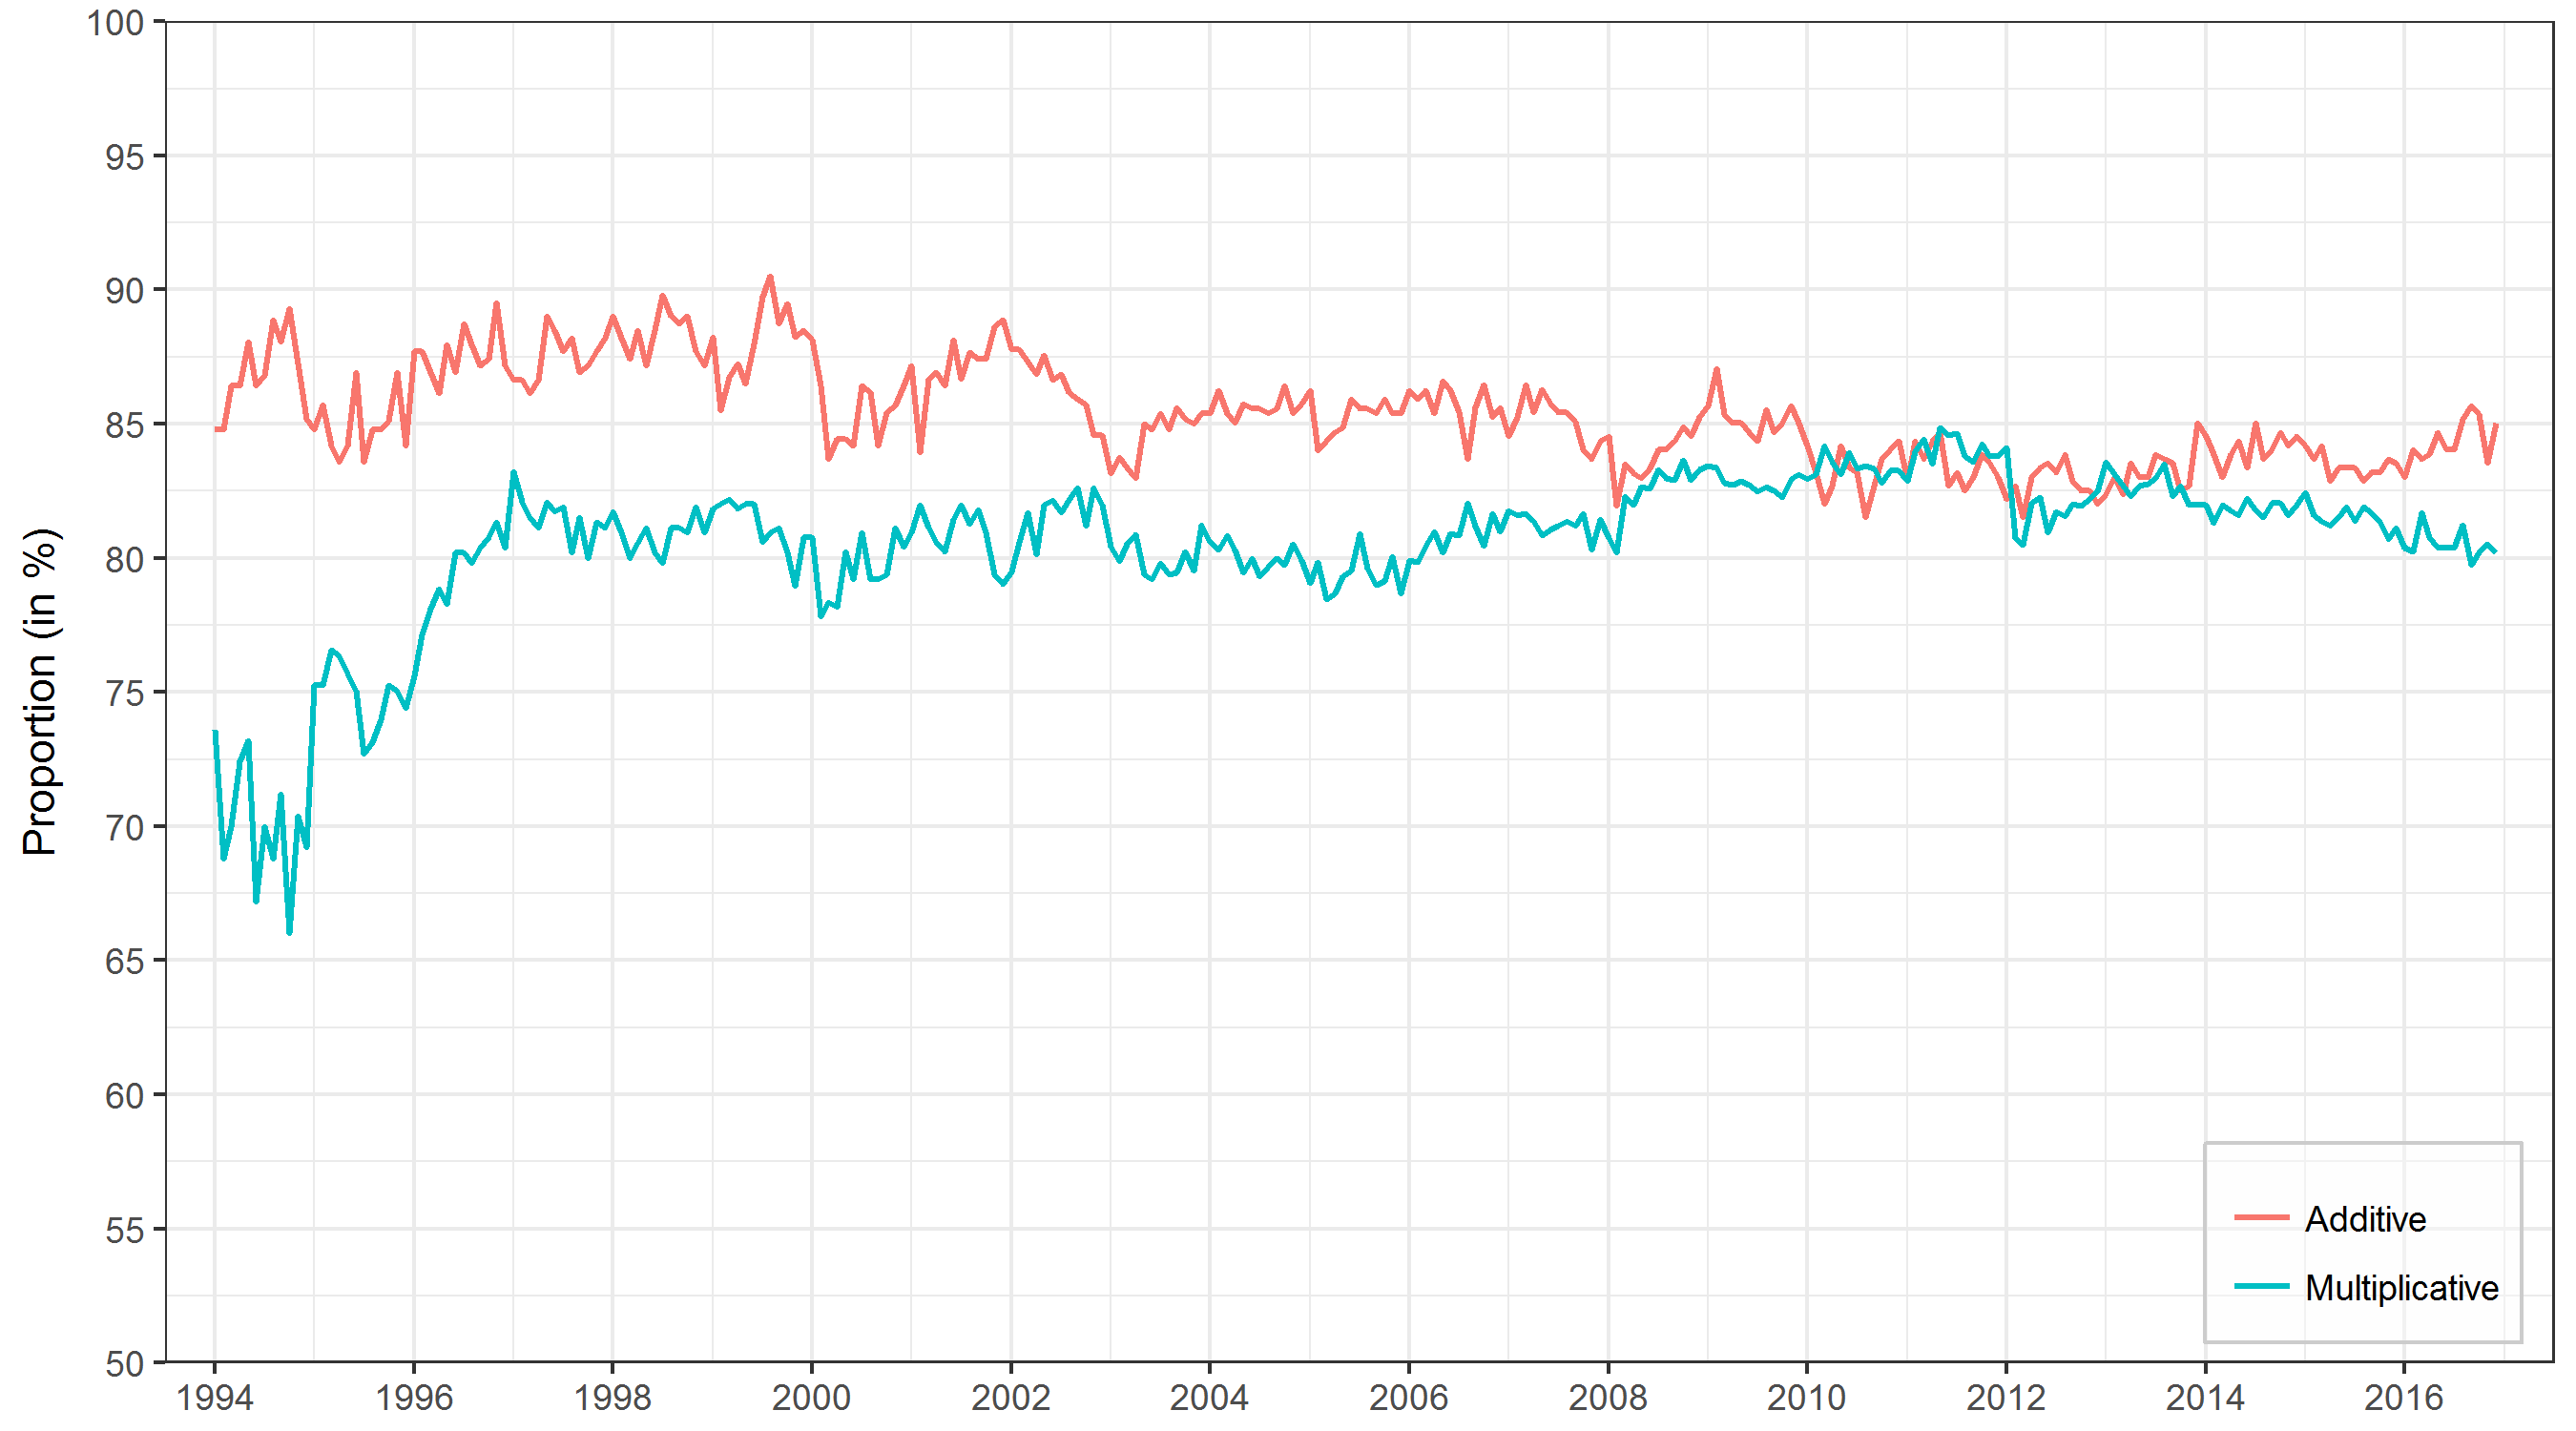
\includegraphics[scale=0.65]{img/LYaicc.png}
 \caption[Change of the percentage of series for which the manual leap year pre-adjustment is better (in terms of $AICC$) than the Reg-ARIMA pre-adjustment (study on 2198 series)]{
Change of the percentage of series for which the manual leap year pre-adjustment is better (in terms of $AICC$) than the Reg-ARIMA pre-adjustment (study on 2198 series).}
 \label{fig:LYaicc}
\end{center}
\end{figure}

\clearpage

\section{Breaks estimate}
\label{sec:AO}

In this section, we study the estimate of outliers and breaks defined in the subsection \ref{sec:PAR}, and more precisely additive outliers ($AO$), level shifts ($LS$), transitory changes ($TC$), seasonal outliers ($SO$).

\subsection{Methodology}

We use the monthly volume indices of the industrial production of the countries of the European community at the four-digit level of NACE rev 2. We only keep the first 12 years of the series to study the convergence of the estimates.
The methodology chosen is very similar to that followed in the previous section. However, to compare the results more easily, the series are corrected from the atypical points in the year of the introduction of the break and they are all rebased to 100 the month of its introduction.
\begin{enumerate}
	\item The decomposition model, atypical points, breaks, trading day effects and the ARIMA model are identified and estimated for the entire series (12 years). The Reg-ARIMA model is therefore determined.
	\item The raw series is corrected for atypical points in the year of introduction of the break and is rebased to 100 at the month of the introduction of the break ($49^{\mbox{\tiny th}}$ observation). These operations do not modify the Reg-ARIMA model, even if, in the case of an additive schema, the rebasing implies a modification of the estimated coefficients which are multiplied by the rebasing coefficient.
	\item We simulate a break at the $49^{\mbox{\tiny th}}$ observation of the series, adding to the series the corresponding regressor multiplied by 10 if the model is additive or by 1.1 if it is multiplicative.
	\item The regressor related to the studied break is added to the Reg-ARIMA model and its coefficient is estimated on the first 49 observations of the series by freezing all the other parameters estimated in the first step.
	\item Finally, the process is repeated by adding an observation each time, which gives new estimates of the parameters. For a 12-year series, we will have $12\times12 - 48 = 96$ estimates of the coefficient of the regressor modeling the break.
\end{enumerate}
These simulations then make it possible to study the convergence of the estimate of the coefficient of the break. In this study, we will say that the estimate of the coefficient of the break has converged when it remains less than 5\% in absolute value of the last estimate.

\subsection{Results}

\begin{figure}[!hb]
\begin{center}
 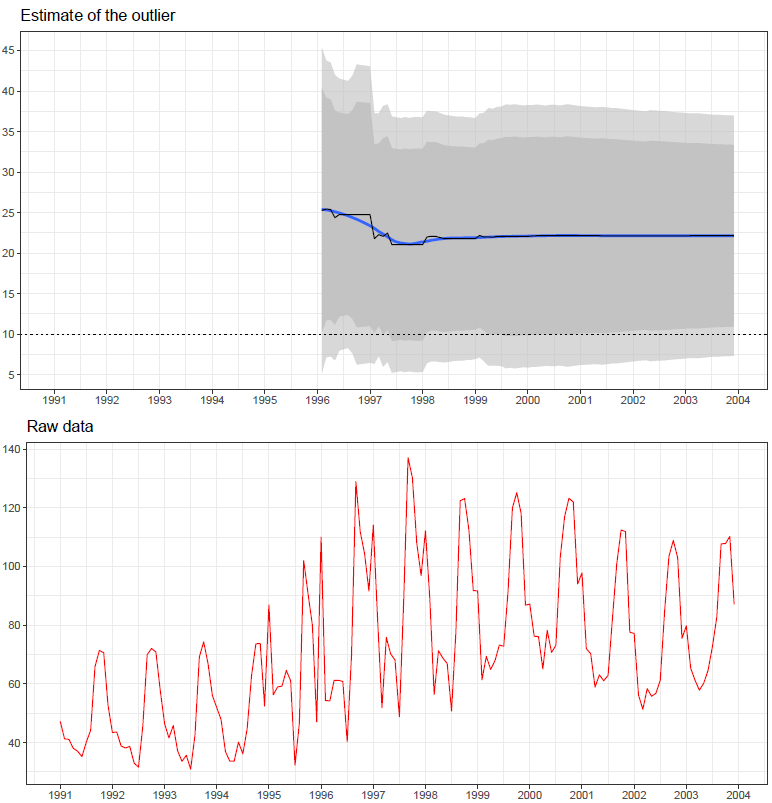
\includegraphics[width=16cm]{img/DE-C1062-EstimateAO.PNG}
 \caption[Raw series and change of the estimate of the additive outlier AO1996.jan for the series DE-C1062 (additive model)]{Raw series and change of the estimate of the additive outlier AO1996.jan for the series DE-C1062 (additive model).}
 \label{fig:DE-C1062}
\end{center}
\end{figure}

\begin{figure}[!ht]
\begin{center}
 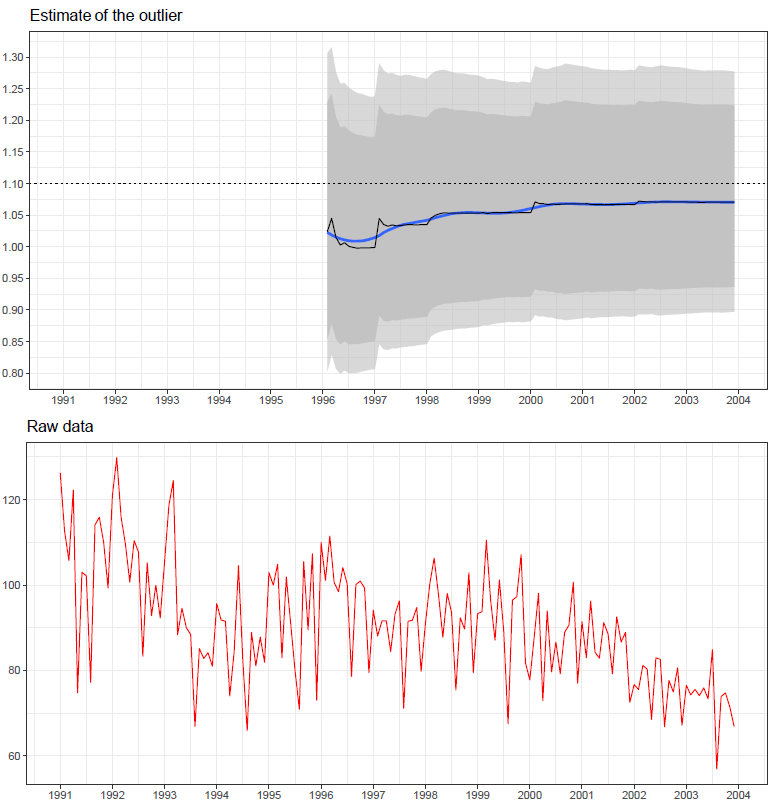
\includegraphics[width=16cm]{img/DE-C1086-EstimateAO.PNG}
 \caption[Raw series and change of the estimate of the additive outlier AO1996.jan for the series DE-C1086 (multiplicative model)]{Raw series and change of the estimate of the additive outlier AO1996.jan for the series DE-C1086 (multiplicative model).}
 \label{fig:DE-C1086}
\end{center}
\end{figure}

The results are shown in figures \ref{fig:DE-C1062} and \ref{fig:DE-C1086}; in these figures, the red curve represents the estimates, the blue curve is a smoothed version, the shaded areas represent the 95\% and 99\% confidence intervals and the dotted line is the real value of the break.
\begin{itemize}
	\item In both cases, the coefficient of the AO takes time to converge and the estimate values of the first years can be quite erratic.
	\item The estimate value can be very different from the real value.
\end{itemize}

\vspace{2mm}

The figures \ref{fig:OutliersConvergence} and \ref{fig:OutliersValue}, as well as theassociated tables \ref{table:AOconvergence} and\ref{table:AOvaleur}, summarize the distributions of the time convergence and the estimated value, for 461 series and the 4 types of breaks studied:
\begin{itemize}
	\item In general, estimates take a long time to converge.
		\item For additive models and 75\% des séries, $SO$, $LS$ and $TC$ take about 7 to converge, 5 years for $AO$. In median, $AO$ and $TC$ take 4 years to converge and $LS$ and $SO$ 5 years.
	\item Convergence seems  slower for multiplicative models since for 75\% of series, $AO$ take about 6 years to converge and $SO$, $LS$ and $TC$ about 7 years. However, in median, $AO$, $LS$, $TC$ and $SO$ converge in 4 years.
	\item In median, the estimates of the different breaks converge approximately to the expected value. But in 50\% of the cases, the estimated value converges to a value around $\pm$ 30\% of the real value. We can also note the presence of abnormal estimates, some of which even show declines instead of the increase modeled.
\end{itemize}

\begin{figure}[h!]
\begin{center}
 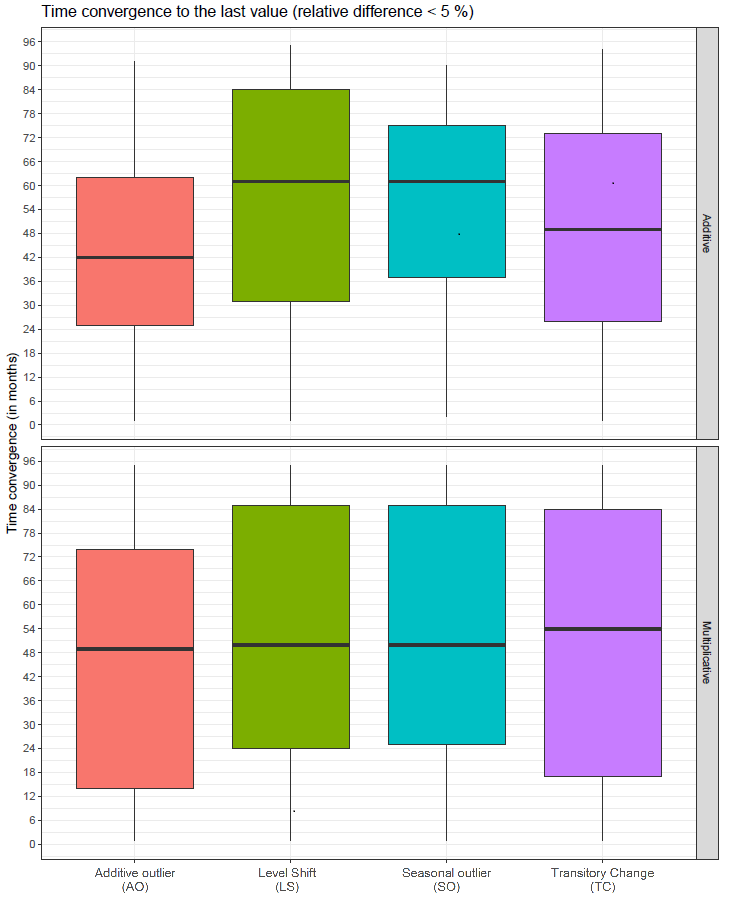
\includegraphics[scale=0.65]{img/OutliersConvergence.png}
 \caption[Time convergence (in months) of the coefficient of the break by the decomposition model]{Time convergence (in months) of the coefficient of the break by the decomposition model.}
 \label{fig:OutliersConvergence}
\end{center}
\end{figure}

\begin{figure}[!ht]
\begin{center}
 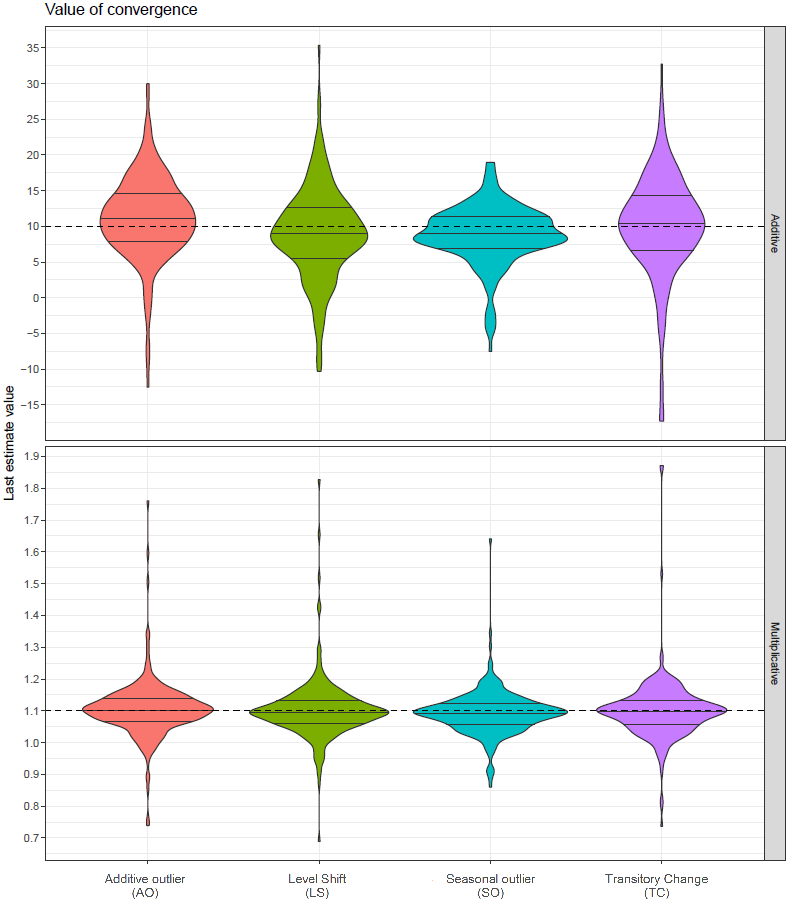
\includegraphics[scale=0.65]{img/OutliersValue.png}
 \caption[Final estimate of the coefficient of the coefficient of the break by the decomposition model]{Final estimate of the coefficient of the coefficient of the break by the decomposition model.}
 \label{fig:OutliersValue}
\end{center}\vspace{-0.3cm}
\footnotesize%
\emph{%
Reading note: on the ordinate, the probability density of the estimate coefficient of the studied breaks. The horizontal lines represent the associated quartiles (minimum, first quartile, median, third quartile and maximum).}
\end{figure}

\clearpage

\begin{table}[h]
\caption[Statistics on the time convergence (in months) of the coefficient of the break by the decomposition model and the type of break]{Statistics on the time convergence (in months) of the coefficient of the break by the decomposition model and the type of break.} \label{table:AOconvergence}
\begin{center}
\begin{tabular}{lccccc}
\toprule
  & Minimum & 25 \% & 50\% & 75\% & Maximum\\
\midrule
\addlinespace[0.3em]
\multicolumn{6}{l}{\textbf{Additive models}}\\
\hspace{1em}AO & 1 & 25 & 42 & 62 & 91\\
\hspace{1em}LS & 1 & 31 & 61 & 84 & 95\\
\hspace{1em}SO & 2 & 37 & 61 & 75 & 90\\
\hspace{1em}TC & 1 & 26 & 49 & 73 & 94\\
\addlinespace[0.3em]
\multicolumn{6}{l}{\textbf{Multiplicative models}}\\
\hspace{1em}AO & 1 & 14 & 49 & 74 & 95\\
\hspace{1em}LS & 1 & 24 & 50 & 85 & 95\\
\hspace{1em}SO & 1 & 25 & 50 & 85 & 95\\
\hspace{1em}TC & 1 & 17 & 54 & 84 & 95\\
\bottomrule
\end{tabular}
\end{center}
\end{table}

\begin{table}[h]
\caption[Statistics on the convergence values by the decomposition model and the type of break. Expected values are +10 for additive models and 1.1 (+10\%) for multiplicative models]{Statistics on the convergence values by the decomposition model and the type of break. Expected values are +10 for additive models and 1.1 (+10\%) for multiplicative models.}\label{table:AOvaleur} 
\begin{center}
\begin{tabular}{lccccc}
\toprule
  & Minimum & 25\% & 50\% & 75\% & Maximum\\
\midrule
\addlinespace[0.3em]
\multicolumn{6}{l}{\textbf{Additive models}}\\
\hspace{1em}AO & -11.6 & 7.8 & 11.1 & 14.2 & 36.9\\
\hspace{1em}LS & -11.4 & 5.6 & 9.3 & 12.7 & 49.8\\
\hspace{1em}SO & -5.8 & 7.3 & 8.8 & 11.0 & 31.1\\
\hspace{1em}TC & -17.4 & 6.5 & 10.2 & 14.1 & 47.2\\
\addlinespace[0.3em]
\multicolumn{6}{l}{\textbf{Multiplicative models}}\\
\hspace{1em}AO & 0.72 & 1.07 & 1.10 & 1.14 & 1.88\\
\hspace{1em}LS & 0.68 & 1.07 & 1.10 & 1.13 & 1.81\\
\hspace{1em}SO & 0.86 & 1.06 & 1.10 & 1.12 & 1.40\\
\hspace{1em}TC & 0.73 & 1.06 & 1.10 & 1.14 & 1.87\\
\bottomrule
\end{tabular}
\end{center}
\end{table}


\clearpage

\section{Estimate of the ARIMA model}

In the proposed example, the series follows an additive model and the general Reg-ARIMA model is:
\begin{eqnarray}
	\label{eq:eq4}
z_t=\beta_0 LY_t + \sum_{j=1}^{j=6} \beta_j \left(N_{jt} - N_{7t}\right) + \sum_{l=1}^{l=k} \alpha_l O_{lt} + x_t,
\end{eqnarray}
where $O_l$ ($l=1,\, \ldots, k$) correspond to the possible breakd detected by the algorithm. In this formulation we can:
\begin{enumerate}
	\item Either let the leap year regressors in the trading days set of regressors automatically generated by the algorithm;
	\item Or remove the leap year from this set and introduce it as an external regressor.
\end{enumerate}
Both models are perfectly equivalent from the theoretical point of view. But the algorithms, implementation of the theory, are not the theory! Indeed, estimates of the same model under slightly different conditions may yield to significantly different results. Thus, if we experiment on the RF241 series of the French IPI, we obtain (figure \ref{fig:CholeskyRF241}):
\begin{itemize}
	\item In the case where the leap year is modeled in the trading days regressors: a significant leap year effect (at the 5\% threshold), calendar effects (working days and leap year effect) are significant (at the 5\% threshold), 3 breaks and an ARIMA model $(2,0,0)(0,1,1)$;
	\item And in the case where the leap year is considered as an external regressor: a significant leap year effect (at the 5\% threshold), no working days effect, 8 breaks and an ARIMA model $(0,1,1)(0,1,1)$.
\end{itemize}

Fortunately this surprising phenomenon is relatively rare. It is due to the fact that in the second case the model is poorly specified: by not introducing the leap year regressor in the calendar effects, they are considered significantly equals to 0 and are therefore not retained by the algorithm. The result is a different ARIMA model and different breaks.

\begin{figure}[!ht]
\begin{center}
 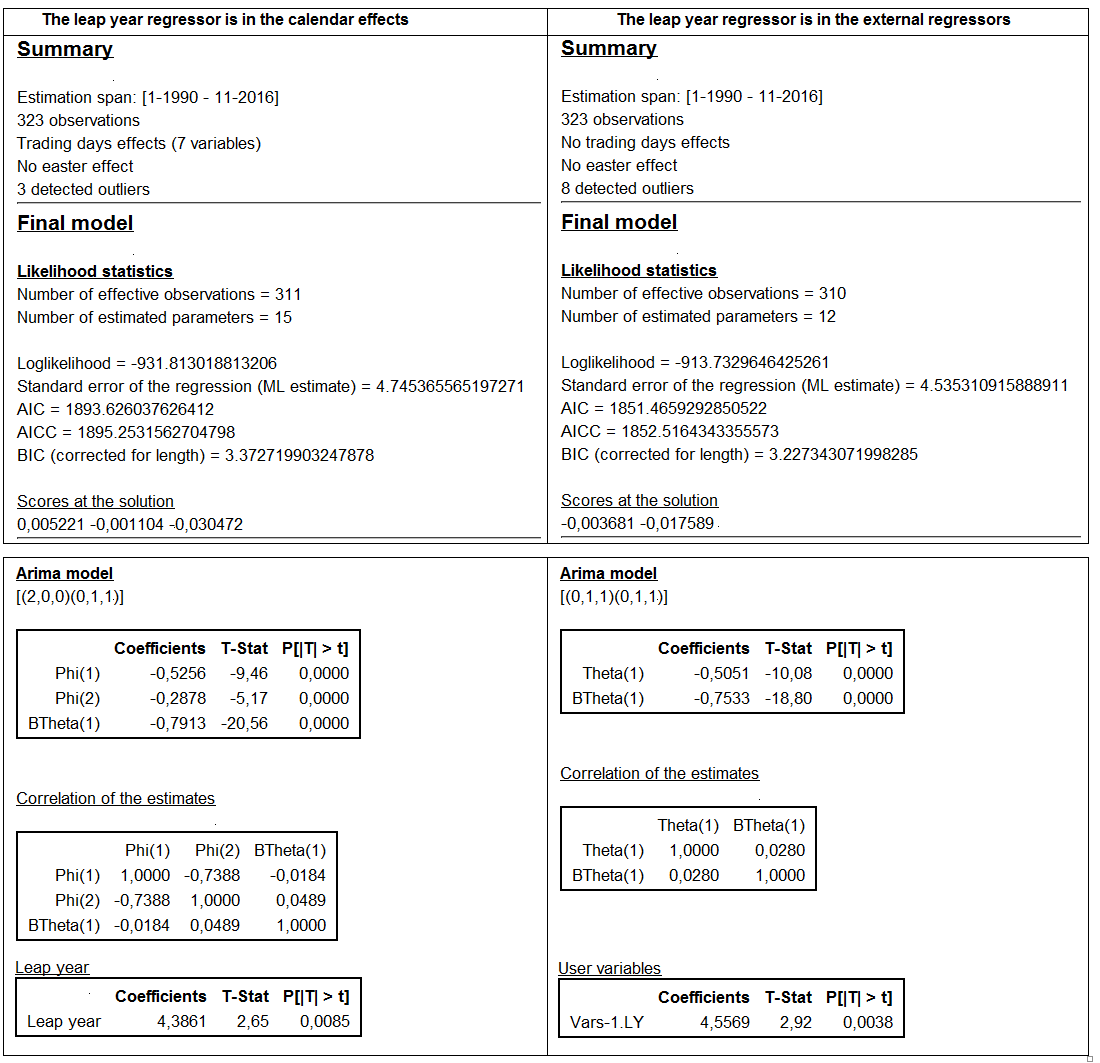
\includegraphics[width=16cm]{img/CholeskyRF241.png}
 \caption[Comparison of the models obtained for the RF241 according to whether the leap year regressor is used or not as an external regressor]{Comparison of the models obtained for the RF241 according to whether the leap year regressor is used or not as an external regressor.}
 \label{fig:CholeskyRF241}
\end{center}
\end{figure}


\clearpage

\section*{Conclusion \markboth{Conclusion}{Conclusion}}
\addcontentsline{toc}{section}{Conclusion}

Reg-ARIMA models are parametric models that, like many parametric methods, are very sensitive to atypical values and to the respect of the assumptions on which they are based. This lack of robustness has been known for decades and is at the origin of the robust statistics (see for example \cite{T1977} and \cite{HR2011}).

To use them well, it is essential to correctly specify \textbf{beforehand} the model and to check that the assumptions of the model are well fulfilled. Therefore:
\begin{itemize}
  \item even if users are fond of long series, it is extremely unlikely that an economic series follows the same ARIMA model for more than 15 years. In particular, the rebasements and changes of nomenclature often lead to retropolize the series with indicators close but with a probable different dynamic. A long series must therefore be seasonally adjusted by sub-periods --- see in this respect \cite{E2015} and \cite{PQLT2018};
	\item an Easter effect on series of industrial production is very unlikely, except perhaps for some very precise levels of nomenclature;
	\item the set of trading days regressors must be based on economic reasons rather than statistical considerations (see the leap year effect example). In this respect, it is interesting to note that the default set of regressors propose by the current methods (6 regressors, one for each day of the week, or 1 regressor representing the 5 days of the week except weekend) are either unstable or inadequate as shown by \cite{A2012} or \cite{L2018}.
\end{itemize}

\vskip \baselineskip
In terms of seasonal adjustment, most of the instabilities mentioned will have a limited effect on the seasonally and trading days adjusted series\footnote{Particularly because the AO, LS and TC are reintroduced into the seasonally adjusted series at end of the process and because calendar effects are usually low.}, especially if \textsc{X-13Arima-Seats} is used. But they will undoubtedly change the story in the short term and eventually introduce unpleasant revisions.

\vskip \baselineskip
The simulations presented in this study are certainly criticizable and improvable but they have the merit of highlighting the potential instability of these Reg-ARIMA models often used as black boxes. However, the automatic algorithms implemented in \textsc{X-13Arima-Seats} and \textsc{Tramo-Seats} are important and very useful tools. The best is certainly to use them in accordance with the ``European guidelines for seasonal adjustment'' published by \cite{E2015}.

Basing, for example, on these models procedures for choosing trading days regressors or more generally for seasonal adjustment parameters, without relying on economic reasoning and knowledge of the field studied, would be a big mistake\dots{} which would probably lead to say about you: \textit{``He uses statistics as a drunken man uses lamp posts, for support rather than illumination''}\footnote {Quote widely attributed to Andrew Lang (1844-1912), Scottish writer, but the original quote has never been found.}

\newpage
\appendix
\section{Le calendrier grégorien}
\label{sec:cal}

Le calendrier grégorien est un calendrier solaire, basé sur le mouvement de la Terre autour du Soleil, et pour lequel l'année est une approximation de l'année tropicale, durée que la Terre prend pour aller d'un point fixe, comme un équinoxe ou un solstice, au suivant. Dans ce calendrier, une année normale est faite de 12 mois --- janvier, février, mars, avril, mai, juin, juillet, août, septembre, octobre, novembre et décembre --- qui contiennent un nombre de jours égal respectivement à 31, 28, 31, 30, 31, 30, 31, 31, 30, 31, 30 et 31. Une année normale contient donc 365 jours, ce qui est malheureusement un peu trop court dans la mesure où la Terre met environ 365 jours et 6 heures pour accomplir une révolution autour du soleil. Une meilleure approximation de l'année solaire est obtenue en ajoutant 1 jour à certaines années, les années bissextiles, pour lesquelles le mois de février aura 29 jours. Une année bissextile est une année divisible par 4 mais pas par 100, sauf si elle est divisible par 400. Ainsi, 1900 ne fut pas une année bissextile, 2000 en était une et 2100 ne sera pas bissextile. On a donc \emph{in fine} 97 années bissextiles sur une période de 400 ans. Il reste cependant une petite erreur d'approximation d'environ 1 jour tous les 4000 ans que le calendrier grégorien ne prend pas en compte.

Toute période de 400 ans contient donc $400 \times 365 + 97 = 146097$ jours, soit exactement $20871$ semaines. Le calendrier grégorien est donc périodique de période 400 ans. La longueur moyenne d'une année sur ce cycle est de $146097 / 400 = 365,2425$ jours et la longueur moyenne d'un mois est de $365,2425 / 12 = 30,436875$ jours.

\newpage
 
\nocite{*}
\begin{thebibliography}{999}
\bibitem[Attal-Toubert (2012)]{A2012} Attal-Toubert, K. (2012), Régresseurs pour effets de calendrier : comment les construire, comment les choisir ? Actes des $11^{\mbox{\tiny èmes}}$ Journées de Méthodologie Statistique, \url{http://jms-insee.fr/jms2012s14_3/}.
\bibitem[Bell (1992)]{B1992} Bell, W. R. (1992), Alternative Approaches to Length of Month Adjustment, Research Report Series 1992-17, Satistical Research Division, U. S. Census Bureau, Washington DC. \url{https://www.census.gov/ts/papers/rr92-17.pdf}.
\bibitem[Eurostat (2015)]{E2015} Eurostat (2015), The ESS guidelines for seasonal adjustment, Eurostat manuals and guidelines, Product Code: KS-GQ-15-001. \url{http://ec.europa.eu/eurostat/web/products-manuals-and-guidelines/-/KS-GQ-15-001}.
\bibitem[Findley and McElroy (2018)]{FMcE2018} Findley, D., McElroy, T. (2018), Background and Perspectives for ARIMA Model-Based Seasonal Adjustment, in Handbook on Seasonal Adjustment, edited by G. L. Mazzi, co-edited by D. Ladiray, European Union, Luxembourg. \url{ec.europa.eu/eurostat/web/products-manuals-and-guidelines/-/KS-GQ-18-001}.
\bibitem[Findley and al. (1998)]{FMBOC1998} Findley, D.F., Monsell, B.C., Bell, W.R., Otto, M.C., Chen, B.C. (1998), New capabilities and methods of the X-12-ARIMA seasonal adjustment program, Journal of Business and Economic Statistics, 16, 127-152.
\bibitem[G\'{o}mez and Maravall (1996)]{GM1996} G\'{o}mez, V. and Maravall, A. (1996), Programs TRAMO and SEATS. Instructions for the User, (with some updates), Working Paper 9628, Servicio de Estudios, Banco de Espa\~{n}a.
\bibitem[G\'{o}mez and Maravall (1998)]{GM1998} G\'{o}mez, V., Maravall, A. (1998), Automatic Modeling Methods For Univariate Series, Working Paper 9808, Servicio de Estudios, Banco de Espa\~{n}a.
\bibitem[Grudkowska (2017)]{G2017} 	Grudkowska, S. (2017),	JDemetra+ Reference Manual Version 2.2, available from URL: \url{https://ec.europa.eu/eurostat/cros/content/software-jdemetra_en}.
\bibitem[Huber and Ronchetti (2011)]{HR2011} Huber, P. J., Ronchetti, E. M. (2011), Robust Statistics, Wiley Series in Probability and Statistics, John Wiley and Sons.
\bibitem[Ladiray and Quenneville (2001)]{LQ2001} Ladiray, D., Quenneville, B. (2001), Seasonal Adjustment with the X-11 Method, Lecture Notes in Statistics No 158, Springer, New York. Available in French on \url{https://www.census.gov/ts/papers/x11_french.pdf}.
\bibitem[Ladiray (2018)]{L2018} Ladiray, D. (2018), Calendar effects, in Handbook on Seasonal Adjustment, edited by G. L. Mazzi, co-edited by D. Ladiray, European Union, Luxembourg. \url{ec.europa.eu/eurostat/web/products-manuals-and-guidelines/-/KS-GQ-18-001}.
\bibitem[Maravall and Caporello (2004)]{MC2004} Maravall, A., Caporello, G. (2004), Program TSW: Revised reference manual. Technical Report, Research Department, Bank of Spain.
\bibitem[Maravall and al. (2015)]{MLP2015} Maravall, A., L\'{o}pez, R., and P\'{e}rez, D. (2015), Reliability of the Automatic Identification of ARIMA Models in Program TRAMO, in Beran, J., Feng, Y., and Hebbel, H. (eds.) Empirical Economic and Financial Research. Theory, Methods and Practice, Springer International Publishing, Switzerland, 105-122.
\bibitem[Maravall and al. (2016)]{MLP2016} Maravall, A., L\'{o}pez, R., and P\'{e}rez, D. (2016), Reg-ARIMA Model Identification: Empirical Evidence, Statistica Sinica, 26, 1365-1388.
\bibitem[Maravall (2018)]{M2018} Maravall, A. (2018), Quality of Seasonal Adjustment in the Model-Based Approach of TRAMO-SEATS, in Handbook on Seasonal Adjustment, edited by G. L. Mazzi, co-edited by D. Ladiray, European Union, Luxembourg. \url{ec.europa.eu/eurostat/web/products-manuals-and-guidelines/-/KS-GQ-18-001}.
\bibitem[Mehrhoff (2018)]{Me2018} Mehrhoff, J. (2018), Outlier Detection and Correction, in Handbook on Seasonal Adjustment, edited by G. L. Mazzi, co-edited by D. Ladiray, European Union, Luxembourg. \url{ec.europa.eu/eurostat/web/products-manuals-and-guidelines/-/KS-GQ-18-001}.
\bibitem[Pham and Quartier-la-Tente (2018)]{PQLT2018} Pham, H., Quartier-la-Tente, A. (2018), Désaisonnaliser les séries très longues par sous-période, gains et choix de la longueur de traitement --- exemple des séries de l'IPI, Actes des $13^{\mbox{\tiny èmes}}$ Journées de Méthodologie Statistique. 
\bibitem[Tukey (1977)]{T1977} Tukey, J. W. (1977), Exploratory Data Analysis, Addison-Wesley Publishing Company.





\end{thebibliography}

%\bibliography{DB}

\end{document}  